%%% Local Variables:
%%% mode: latex
%%% TeX-master: t
%%% End:

\documentclass[bachelor,nofonts]{thuthesis}
%\documentclass[master]{thuthesis}
%\documentclass[doctor]{thuthesis}
% \documentclass[%
%   bachelor|master|doctor|postdoctor, % mandatory option
%   winfonts|nofonts|adobefonts, % mandatory only for bachelor and Linuxer
%   secret,
%   openany|openright,
%   arialtoc,arialtitle]{thuthesis}
% 当使用 XeLaTeX 编译时,本科生、Linux 用户需要加上 nofonts 选项;
% 当使用 PDFLaTeX 编译时,adobefonts 选项等效于 winfonts 选项(缺省选项)。

% 所有其它可能用到的包都统一放到这里了,可以根据自己的实际添加或者删除。
\usepackage{thutils}
\usepackage{listings}
\usepackage{float}
\usepackage{color}
\usepackage{xcolor}
\usepackage{tikz}
\usetikzlibrary{shapes,arrows,shadows,decorations.markings,fit,positioning}
\usepackage{amsmath,bm,times}
%\usepackage{pgf-umlsd}
\usepackage[underline=true,rounded corners=false]{pgf-umlsd}
\usepackage{fancyvrb}

% Define the layers to draw the diagram
\pgfdeclarelayer{background}
\pgfdeclarelayer{foreground}
\pgfsetlayers{background,main,foreground}
\tikzstyle{sensor}=[draw, fill=blue!20, text width=2em, 
    text centered, minimum height=2.5em,drop shadow]

\definecolor{mygreen}{rgb}{0,0.6,0}
\definecolor{mygray}{rgb}{0.5,0.5,0.5}
\definecolor{mymauve}{rgb}{0.58,0,0.82}

\lstset{ %
  backgroundcolor=\color{white},   % choose the background color; you must add \usepackage{color} or \usepackage{xcolor}
  %basicstyle=\footnotesize,        % the size of the fonts that are used for the code
  basicstyle=\ttfamily\small, 
  commentstyle=\ttfamily\small,
  breakatwhitespace=false,         % sets if automatic breaks should only happen at whitespace
  breaklines=true,                 % sets automatic line breaking
  commentstyle=\color{mygreen},    % comment style
  extendedchars=true,              % lets you use non-ASCII characters; for 8-bits encodings only, does not work with UTF-8
  frame=shadowbox,                    % adds a frame around the code
  rulesepcolor=\color{red!20!green!20!blue!20},
  keepspaces=true,                 % keeps spaces in text, useful for keeping indentation of code (possibly needs columns=flexible)
  keywordstyle=\color{blue},       % keyword style
  language=c++,                 % the language of the code
  %numbers=left,                    % where to put the line-numbers; possible values are (none, left, right)
  numbersep=5pt,                   % how far the line-numbers are from the code
  numberstyle=\tiny\color{mygray}, % the style that is used for the line-numbers
  rulecolor=\color{black},         % if not set, the frame-color may be changed on line-breaks within not-black text (e.g. comments (green here))
  showspaces=false,                % show spaces everywhere adding particular underscores; it overrides 'showstringspaces'
  showstringspaces=false,          % underline spaces within strings only
  showtabs=false,                  % show tabs within strings adding particular underscores
 % stepnumber=2,                    % the step between two line-numbers. If it's 1, each line will be numbered
  stringstyle=\color{mymauve},     % string literal style
  tabsize=2,                       % sets default tabsize to 2 spaces
linewidth=\textwidth,
xleftmargin=0.05\textwidth,
xrightmargin=0.05\textwidth,
  title=\lstname                   % show the filename of files included with \lstinputlisting; also try caption instead of title
}

\floatstyle{plain} % optionally change the style of the new float
\newfloat{Code}{H}{myc}

% 你可以在这里修改配置文件中的定义,导言区可以使用中文。
% \def\myname{陈宇恒}

\renewcommand\lstlistingname{代码}
\begin{document}

% 定义所有的eps文件在 figures 子目录下
\graphicspath{{figures/}}


%%% 封面部分
\frontmatter

%%% Local Variables:
%%% mode: latex
%%% TeX-master: t
%%% End:
%\secretlevel{绝密} \secretyear{2100}

\ctitle{多核可扩展操作系统内核关键技术的研究与实现}
% 根据自己的情况选,不用这样复杂
\makeatletter
\ifthu@bachelor\relax\else
  \ifthu@doctor
    \cdegree{工学博士}
  \else
    \ifthu@master
      \cdegree{工学硕士}
    \fi
  \fi
\fi
\makeatother


\cdepartment[计算机]{计算机科学与技术系}
\cmajor{计算机科学与技术}
\cauthor{陈宇恒} 
\csupervisor{陈渝~副教授}
% 如果没有副指导老师或者联合指导老师,把下面两行相应的删除即可。
%\cassosupervisor{陈文光教授}
%\ccosupervisor{某某某教授}
% 日期自动生成,如果你要自己写就改这个cdate
%\cdate{\CJKdigits{\the\year}年\CJKnumber{\the\month}月}

% 博士后部分
% \cfirstdiscipline{计算机科学与技术}
% \cseconddiscipline{系统结构}
% \postdoctordate{2009年7月——2011年7月}

\etitle{TODO: Implementation and Analysis of Operating System on Multicore
System} 
% 这块比较复杂,需要分情况讨论:
% 1. 学术型硕士
%    \edegree:必须为Master of Arts或Master of Science(注意大小写)
%              “哲学、文学、历史学、法学、教育学、艺术学门类,公共管理学科
%               填写Master of Arts,其它填写Master of Science”
%    \emajor:“获得一级学科授权的学科填写一级学科名称,其它填写二级学科名称”
% 2. 专业型硕士
%    \edegree:“填写专业学位英文名称全称”
%    \emajor:“工程硕士填写工程领域,其它专业学位不填写此项”
% 3. 学术型博士
%    \edegree:Doctor of Philosophy(注意大小写)
%    \emajor:“获得一级学科授权的学科填写一级学科名称,其它填写二级学科名称”
% 4. 专业型博士
%    \edegree:“填写专业学位英文名称全称”
%    \emajor:不填写此项
\edegree{TODO DEGREE} 
\emajor{Computer Science and Technology} 
\eauthor{Chen Yuheng} 
\esupervisor{Associate Professor Chen Yu} 
%\eassosupervisor{Chen Wenguang} 
% 这个日期也会自动生成,你要改么?
% \edate{December, 2005}

% 定义中英文摘要和关键字
\begin{cabstract}

随着多核架构计算机技术的迅猛发展,如何使用新方法提高操作系统内核的多核可扩展性性能,已经成
为操作系统领域关注的重要课题,具有较高的研究价值和现实意义。
本文的主要工作包括:对Linux 虚拟内存管理系统的多核竞争瓶颈问题和MIT提出的RadixVM相关多核优化技术
进行了深入研究;基于RadixVM提出了一种针对对象引用计数器和简化 Posix 标准的操作系统虚
拟内存管理子系统的建模方法,并在可交换性原理的基础上通过KLEE 符号执行引擎设计了
求解操作系统模型中可扩展实现存在条件的方法;基于分析出的可扩展性存在条件设计实现了一个
支持 AMD64 NUMA 多核架构的操作系统内核原型ucore-mp;实现了一款基于 QEMU 模拟器的全系统性能分析工具 QProf,用于方便地测试
操作系统内核性能。实验结果表明,ucore-mp引用技术多核优化技术在多核硬件平台上比一般原子操作的扩展性性能加速比提高了73\%以上。

\end{cabstract}

\ckeywords{操作系统, 符号执行, 多核可扩展性}

\begin{eabstract} 
	
	As the development of microelectronic technology, multicore scalability on hardware systems has become a big challenge to the operating system developers.  Designing new mechanism to improve the multicore scalability is an attractive topic in both industry and academia.
	This paper analyzes the scalability bottleneck in the virtual memory subsystem of Linux, and research into several optimization technology on multicore 
	systems, such as RadixVM from MIT. Based on these technologies, we propose a modeling method for reference counter and
	virtual memory subsystem conforming to a simplified Posix specification.  Furthermore, we combine KLEE symbolic execution engine and the commutability rule 
	to prove the existence of multicore scalable implementations of system interfaces. Based on the theory, we develop a modern operating system kernel ucore-mp on
	AMD64 NUMA multicore  architecture. Finally, a QEMU-based full system profiler QProf is developed to find potential performance problems in the kernel. An Experimental evaluation shows s performance improvements of 73\% or more with ucore-mp reference counter implementation, compared to atomic operations.
\end{eabstract}

\ekeywords{Operating System, Symbolic Execution, Scalability}

% 设置 PDF 文档的作者、主题等属性
\makeatletter
\thu@setup@pdfinfo
\makeatother
\makecover

% 目录
\tableofcontents

% 符号对照表
\begin{denotation}

\item[Cache] 处理器高速缓存
\item[SMP] 对称多处理
\item[NUMA] 非均匀访存模型 (Non-Uniform Memory Access)
\item[OS] 操作系统 (Operating System)
\item[TLB] 旁路转换缓冲 (Translation lookaside buffer)
\item[HPC] 高性能计算 (High Performance Computing)
\item[API] 应用程序编程接口
\item[HAL] 硬件抽象层 (Hardware Abstract Layer)
\item[Perfect Scalibility]
	完美可扩展性,指程序的性能随着CPU核数增加成正比提高
\item[VMM] 虚拟内存管理子系统 (Virtual Memory Management)
\item[VMA] 虚拟内存区域 (Virtual Memory
	Area),Linux等操作系统内部存储虚拟地址映射元数据的对象
\item[RCU]
	Read-Copy-Update机制,一种可以达到比读写锁扩展性更好的同步机制
\item[ACPI] 高级配置和电源管理接口(Advanced Configuration and Power Management Interface)
\item[APIC] 高级可编程中断控制器(Advanced Programmable Interrupt Controller)
\item[LAPIC] 本地高级可编程中断控制器(Local Advanced Programmable Interrupt Controller)
\end{denotation}



%%% 正文部分
\mainmatter

%%% Local Variables:
%%% mode: latex
%%% TeX-master: t
%%% End:

\chapter{引言}

\section{研究背景}

近年来,多核处理器已经成为主流。无论在大型服务器系统,还是在手机、平板电脑等嵌入式系统中,多核硬件都抢占了很大一部分市场。
究其原因,随着半导体制造工艺的提高,极大地缩小了CPU中基本门电路的尺寸,但同时
基于半导体技术的微电子电路已经越来越接近它的物理限制。随着这些物理限制
的临近,CPU的热功耗和数据传输同步问题已经使得通过升高单CPU主频提高系统性能的难度越来越大。尽管研究界和工业界提出了多种方法提高计算机系统的性能:如超标量流水线技术和单指令多数据流(SIMD)技术,但是Web服务器和邮件服务器一类服务器级应用更适合使用多核多进程/多线程模型提高其吞吐量。随着硬件虚拟化技术的成熟,服务器提供商可以轻易地划分单机CPU资源,进一步推动了多核CPU的普及。近年来,无论是在普通家用PC还是服务器,甚至是手机上,设备CPU核数变得越来越多已经成为了一个不可逆转的趋势。

\begin{figure}[ht]
\begin{center}
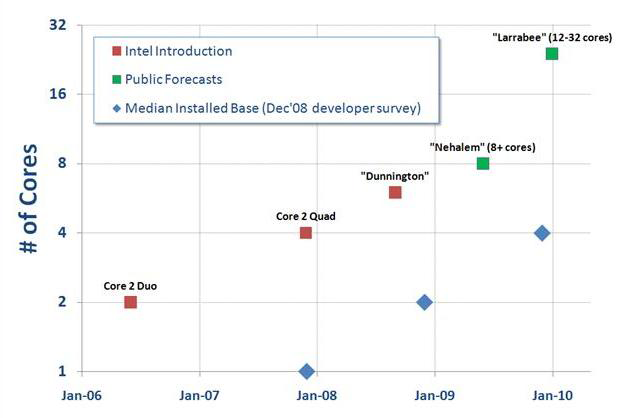
\includegraphics[width=0.7\textwidth]{figures/intro_roadmap.png}
\end{center}
\caption{Intel多核处理器发布计划图\protect\footnotemark}
\label{fig:intro_roadmap}
\end{figure}
\footnotetext{http://software.intel.com/en-us/articles/gaming-into-the-future}

在服务器应用上面,当前基于AMD64/X86\_64架构的多核系统已经得到广泛应用。但随着40核甚至
80核的NUMA系统的出现,对已有操作系统的多核可扩展性能提出了苛刻的要求。
近年越来越多的研究发现\cite{radixvm:eurosys13},由于现有操作系统在设计上的问题,OS在最新的多核系统中成为瓶颈的情况大大增多。例如,目前主流开源操作系统,如Linux和FreeBSD在应对40到80核的NUMA系统时,存在以下问题:

	\begin{itemize}
		\item
	由于已有操作系统多数是由单核系统演化而来,在设计之初就使用了一些
	不具有多核扩展性的数据结构来维护VMA、DCACHE、MountTable等内核关键
	数据结构。这导致Linux等操作系统在20核以上硬件系统上表现不佳,甚至
	出现性能下降\cite{linux:osdi10};
		\item 一些同步原语没有为重核架构优化,例如Linux的Spinlock
			实现在重核架构上导致代价高昂的Cache同步协议开销;
		\item
			操作系统设计上的问题。例如Linux中各个Core共享页表,
			在一些应用下造成不必要的TLB无效化(TLB shootdown)。
	\end{itemize}

由于现有操作系统中存在着以上这些问题,操作系统的虚拟内存管理和文件系统模块经常成为应用程序在多核系统上扩展性的瓶颈。如Exim邮件服务器、Apache
Web服务器和memcached等常用服务器应用在20核对称处理系统或NUMA系统上,常常无法无法达到与CPU核数成正比的加速比(即时在网络、磁盘等输入输出设备性能还没有达到饱和的时候仍然如此),甚至出现随着CPU核数的增加,由于操作系统内部数据竞争情况过于剧烈造成应用程序性能下降的情况\cite{linux:osdi10}。

在服务器应用以外,多核处理器已经在个人数字设备(如智能手机和平板电脑)上推广开来。2012年推出的基于ARM的NVIDIA
Tegra
3四核处理器更加明确了移动设备向多核发展的趋势。对于Linux等跨硬件平台的操作系统,如何建立更高效的多核系统抽象、设计并发友好的无锁无高速缓存竞争的数据结构变得尤为重要。

\section{课题目标}

	鉴于上述的问题,我们希望重新设计一个小型实验性操作系统和相应工具,
	从根本上解决这些问题。重头实现一个操作系统是比较有挑战性的,但我们已有uCore、MIT的xv6/SCK等实验性操作系统做参考。本课题把完成了可扩展多核操作系统实现的基础性工作,以清华大学操作系统研究组编写的uCore教学操作系统为基础,加上对AMD64
	NUMA架构的硬件抽象层(HAL)支持并在QEMU模拟器、KVM硬件虚拟化平台和基于Intel处理器的真实机器上测试通过。在此基础之上,通过模型验证和符号执行的方法,发现操作系统内部的可扩展潜能并用相关数据结构做实现。最后,完成了一种新的基于QEMU的全系统性能测试工具,帮助开发者发现系统可能存在的性能瓶颈。




%%% Local Variables: 
%%% mode: latex
%%% TeX-master: t
%%% End: 

\chapter{相关工作}
\label{cha:relwork}

在现代操作系统研究中,操作系统的多核可扩展性是一个重要研究领域。为了开发多核友好的数据结构和算法,众多研究者已经对Linux内核中的多核优化问题进行了深入研究。例如
MIT PDOS研究组通过修改Linux内自旋锁(spinlock)的API实现\cite{locks:linuxsymp},极大地优化了Linux内核在48核机器上EXIM等应用的性能。下面将对一系列多核优化相关工作进行进一步阐述。

\section{Linux内核多核扩展性研究}
Linux作为服务器系统上应用最广泛的操作系统内核,其多核可扩展性受到广大用户关注。
在学术界和工业界,类Unix操作系统在SMP和NUMA架构上的可扩展性性能研究已经有了很长历史,除了Intel和AMD的多核架构之外,Stanford提出了FLASH研究项目\cite{kuskin1994stanford}、IBM等公司也生产出了几十上百个核的基于共享内存模型的计算机。为了使操作系统在这类硬件上达到良好的可扩展性,可扩展锁、wait-free同步、多核
调度算法、多核内存管理算法等技术被不断提出。这些新技术有的已经在诸如Linux、Solaris等实用操作系统中被广泛应用。

在众多Linux内核研究工作之中,Silas Boyd-Wickizer等人提出了一整套内核可扩展性测试例程Metis\cite{linux:osdi10},发现了Linux中潜在的可扩展性问题并提出了部分解决方案。
在文章中,他们分析了7个重要的系统应用(包括Exim、memcached、Apache、PostgreSQL、gmake、Psearchy和MapReduce)在48核Linux机器上的运行情况。发现除了
gmake之外,所有应用程序都在近期的Linux内核版本中遇到了可扩展性瓶颈。如图\ref{fig:memcached}所示,实验证明,在Linux中随着CPU核数增多,memcached的性能反而下降。

\begin{figure}[ht]
\begin{center}
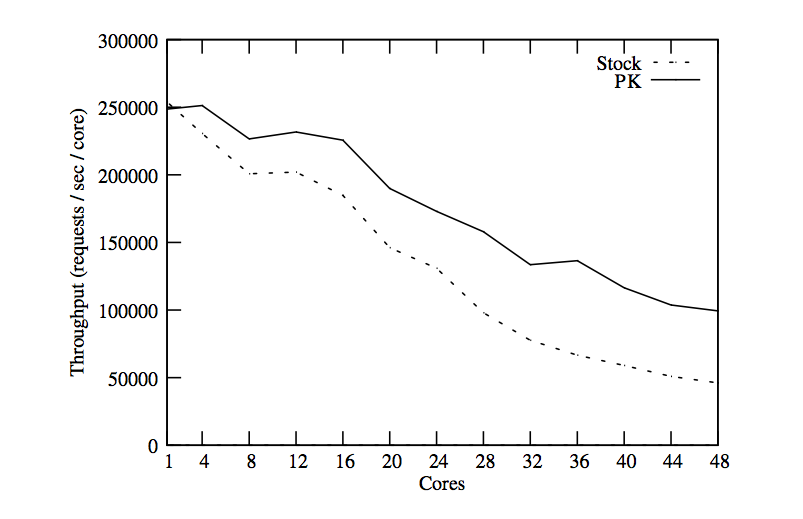
\includegraphics[width=0.7\textwidth]{figures/memcached_test.png}
\end{center}
\caption{memcached吞吐量\cite{linux:osdi10}}
\label{fig:memcached}
\end{figure}

根据已有研究工作造成操作系统扩展性问题的原因总结有:

\begin{itemize}
\item 对共享数据结构加锁,核数增多造成各CPU在核上等待时间变长。
\item 在不同CPU上读写同一内存位置(包括假共享),这会在硬件保证Cache一致性的平台上带来额外的Cache一致性协议开销
\item 多个进程或线程竞争有限的Cache,降低CPU的Cache命中率
\item 多个进程或线程竞争有限的内存带宽
\end{itemize}

从上述几点看以看出,造成操作系统或应用程序在多核平台上性能问题的一个主要原因来自于数据共享,以及为了保护共享数据而
加上的锁。因此,有研究者通过设计新的数据结构管理内核对象,以此减少共享数据带来的开销。此外,文章还总结了10多个造成多核性能瓶颈的关键代码点,
并对Linux做出对于修改。他们修改了Linux2.6.35-rc5,使之在多核平台上性能表现显著提升。

\section{K42实验操作系统}
K42\cite{Krieger:2006:KBC:1218063.1217949}是由IBM公司开发的一个与Linux二进制接口兼容的可扩展操作系统内核。K42在设计之初就考虑到多核硬件上的可扩展性,遵循减少核间数据共享、最大化数据局部性达这一原则。K42的设计者通过以下四项技术优化它的多核可扩展性:
\begin{itemize}
\item 使用客户端-服务器端模型提供系统内核服务。系统服务通过过程调用的方式提供给客户端,客户端的系统服务请求总是有本CPU核上的服务线程处理,避免核间通讯;
\item 感知数据局部性的内存分配器;
\item 面向对象的设计方式。系统服务操作只施加在受影响的对象上,以此限制数据访问的局部性;
\item 使用一个名为Clustered Object的统一模型,对内核对象进行管理。这一编程模型使用分布式系统的方法,提供可扩展的对象冗余(replication)、数据结构和算法划分操作。
\end{itemize}

K42的主要不足是开发时间距今太长,主要面向PowerPC架构,对NUMA系统的支持不够成熟等。

\section{MIT xv6实验操作系统}

在工业界,Linux开发者在不断优化Linux内核对象的数据结构,以求达到在SMP和NUMA系统上达到线性的多核可扩展性能。尽管Linux内核在最新40核以上系统中部分子系统性能表现不佳,但多年来Linux开发者在内核多核性能优化做出的杰出的努力:

\begin{itemize}
\item Linux kernel 2.0引入SMP架构支持;
\item Linux kernel 2.5允许内核抢占(preempt);
\item Linux kernel 2.6.19中引入了当前使用的RCU实现;
\item Linux kernel 2.6.39版本正式移除的内核大锁(Big Kernel
Lock),在此之前大部分Linux的内核态代码不支持同时在多个CPU上运行。
\end{itemize}

但是,Linux在一些重要子系统中还是使用粒度较大的锁来保证内核数据的一致性。最明显的一个子系统就是Linux的虚拟内存管理子系统。mmap和munmap两个系统调用是Linux中使用最频繁的系统调用之一,但是对于每个进程,Linux使用一个大锁来保护其VMA结构体:

\begin{lstlisting}
/* Linux 3.9.2 mm/utils.c */
down_write(&mm->mmap_sem);
ret = do_mmap_pgoff(file, addr, len, prot, flag, pgoff,
		&populate);                        
up_write(&mm->mmap_sem);                               
\end{lstlisting}

如上面代码所示,Linux中对同一进程的mmap调用都加上了锁,实际上串行化了所有虚拟内存分配操作,这成为一些了单进程多线程的应用程序(如Java虚拟机的多线程内存分配器和垃圾回收器)的瓶颈。

为了解决这些问题,学术界提出了各种各样的解决方法,MIT
PDOS研究小组的Austin T. Clements等人提出了多种解决多核操作系统内数据竞争问题的新型数据结构\cite{radixvm:eurosys13}。设计了运行在AMD64平台的操作系统内核xv6。并基于xv6实验OS实现了一个全新的虚拟存储管理模块RadixVM,在80核机器上获得
了几乎线性的加速比。他们主要工作有:
\begin{itemize}
\item 使用Refcache替代传统的原子加减操作
\item 使用改进Radix
Tree实现VMA映射,使得对虚拟地址不重叠的的mmap和munmap操作可以完全并行地进行
\item 跟踪每个CPU内核的内存使用,只对必要的CPU内核进行TLB Shootdown操作
\end{itemize}

相关研究人员在80核的机器上经行了实验,发现RadixVM系统在非重叠虚拟内存区域中达到了完美可扩展。换言之,如果多个线程并行地地经行mmap和munmap系统调用,这些调用可以完全独立运行,并且不会带来Cache一致性协议造成的多核通讯流量。


\section{操作系统接口改进研究}
除了对操作系统内部对象数据结构的改进,也有部分研究把重心放在寻找和优化操作系统对用户程序的接口(主要是系统调用)上。
Baumann等人以此为基础,设计了一个新型的支持异构多核硬件的操作系统Barrelfish\cite{Baumann:2009:MNO:1629575.1629579}。
\begin{figure}[ht]
\centering
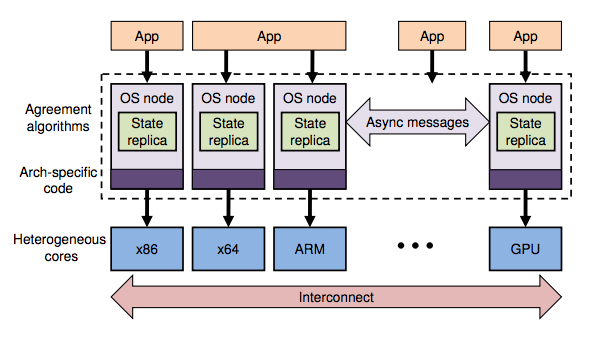
\includegraphics[width=0.7\textwidth]{figures/barrelfish.png}
\caption{Barrelfish系统架构\cite{Baumann:2009:MNO:1629575.1629579}}
\label{fig:barrelfish}
\end{figure}

Barrelfish的开发者认为,把分布式系统中信息传递(Message-Passing)的思想应用到传统操作系统之中。他们认为当前和未来多核硬件会越来越解决于网络系统,这促使我们用分布式系统的思想重新考虑操作系统的设计。因此,他们抛弃过去的基于共享内存的多核操作系统设计方式,把系统中的进程看做发布系统的节点,在它们之间通过信息传递方式交换信息。Baumann等人认为,他们的设计的操作系统Barrelfish(图\ref{fig:barrelfish})比起传统操作系统设计,更容易适应未来多核硬件的发展。

也有研究者通过通过截然不同的方法来挖掘操作系统接口的并行性。有研究者\cite{commuter:2013}通过对操作系统Posix API建模的方法,求解系统调用的可交换性,从而分析不同调用参数和执行路径形成的共享数据依赖关系并寻找潜在的多核可扩展空间。这种方法将在后面的章节仔细讨论。

综上所述,目前多核操作系统的可扩展性研究仍然是目前研究的热点,各国研究机构和公司都在提出各自的操作系统内核解决方案。因此,在最新的多核硬件上实现一个实验用多核可扩展操作系统内核将为以后的操作系统优化工作打下重要的基础。




\chapter{多核操作系统可扩展性分析与建模}

本节将介绍在现代AMD64多核处理器上造成操作系统可扩展性瓶颈的原因。值得注意的是本毕设只考虑由于多核CPU核间通讯开销造成的操作系统性能退化,
一下讨论均忽略系统中其他子系统(如I/O子系统)造成的性能瓶颈。

在造成Linux等现有OS在16核以上多核系统上可扩展性问题的各种因素中,一个核心原因是CPU核间数据共享及其竞争。这种竞争体现在多个方面:

\begin{itemize}
\item 通过原子操作指令(x86中的Lock前缀)修改内核对象的引用计数
(reference count)。由于在x86等体系结构中,一般有已经保证各个核之间的Cache一致性,多个核上使用原子操作修改同一内存地址时,这将迫使
CPU执行Snoop Protocal协议(如在Intel处理器中的QuickPath Interconnect)。在AMD和Intel处理器上Snoop Protocal的复杂度为$O(n)$\cite{intelquickpath},
其中$n$为CPU核数。
当系统中CPU核数增加,各个核上的内存请求将被串行化,这可能会成为操作系统的瓶颈;
\item 通过锁操作控制共享数据访问。为了保证内核中数据结构的一致性,内核需要使用不同粒度的锁保护关键代码段;
\item 通过LAPIC等硬件实现由软件发起的处理器间中断(Interprocessor Interruption)带来的高昂的核间通讯代价。如在多核AMD64系统上,IPI通常被用于发起
TLB无效化请求。
\end{itemize}

下面,我们将使用Linux中虚拟内存子系统作为例子,分析提高操作系统在多核硬件上的可扩展性的重要性和挑战性。

\section{Linux中虚拟内存子系统案例分析}

mmap和munmap两个系统调用是Linux虚拟内存子系统中使用最频繁的系统调用之一,但是对于每个进程,Linux使用一个大锁来保护其VMA结构体:

\begin{lstlisting}
/* Linux 3.9.2 mm/utils.c */
down_write(&mm->mmap_sem);
ret = do_mmap_pgoff(file, addr, len, prot, flag, pgoff,
		&populate);                        
up_write(&mm->mmap_sem);                               
\end{lstlisting}

如上面代码所示,Linux中对同一进程的mmap调用都加上了锁,实际上串行化了所有虚拟内存分配操作,这可能成为频繁调用这两个系统调用分配和释放内存的
多线程应用的瓶颈。事实上,现在Linux中对两个系统调用的实现完全不具有多核可扩展性。事实上,我们可以使用一个简单的程序来验证Linux中mmap系统调用的可扩展性问题:

\begin{lstlisting}
static void *  thread_mmap(void *arg){                                                                                               
	int id = (int)arg;                                                                      
	int c = 0, i;                                                                         
	for(i=0;i<COUNT;i++){                                                                   
		int l = 4096 * (rand() % 5 + 1); 
		void *t = mmap(NULL, l, PROT_WRITE|PROT_READ, 
			MAP_PRIVATE|MAP_ANONYMOUS, -1, 0);
		assert(t != MAP_FAILED);                                                        
		c++;                                                                            
	} 
	counter[id] = c;                                                                        
	return NULL;                                                                            
}                                                                                               
                                                                                                
int main(int argc, const char* argv[]) {                                                                                               
	/* ... */
	for(i=0;i<threads;i++)
		pthread_create(th+i, NULL, thread_mmap, (void*)i);                                                                                
	for(i=0;i<threads;i++)                                                                  
		pthread_join(th[i], (void**)&res); 
	/* ... */
}                                                                                                                          
\end{lstlisting}

在上面的程序中,用mmap系统调用多次向操作系统申请空闲的虚拟地址空间。由于同一进程的多个线程共享同一个地址空间(即同一VMA结构体),这在多核系统上将造成mm->mmap\_sem锁的饱和竞争情况,测试结果如图\ref{fig:mmap_test}所示。应该注意的是,我们调用mmap时使用了MAP\_PRIVATE和MAP\_ANONYMOUS标志,并且不指定addr参数申请固定的虚拟内存地址,操作系统应该有最大的自由度选择适当的虚拟内存区域避免VMA操作的竞争。但从测试结果可以看出,当CPU核数增多时,每秒执行的mmap次数反而降低。这符合Linux代码中VMA结构上由于内核中锁竞争造成应用程序严重性能瓶颈的预期。但是,下面我们将通过对Posix系统调用接口中mmap/munmap和缺页中断的建模,并通过符号执行技术证明Linux中对非重叠区域上VMA全局进程锁是不必要的。

\begin{figure}[ht]
\begin{center}
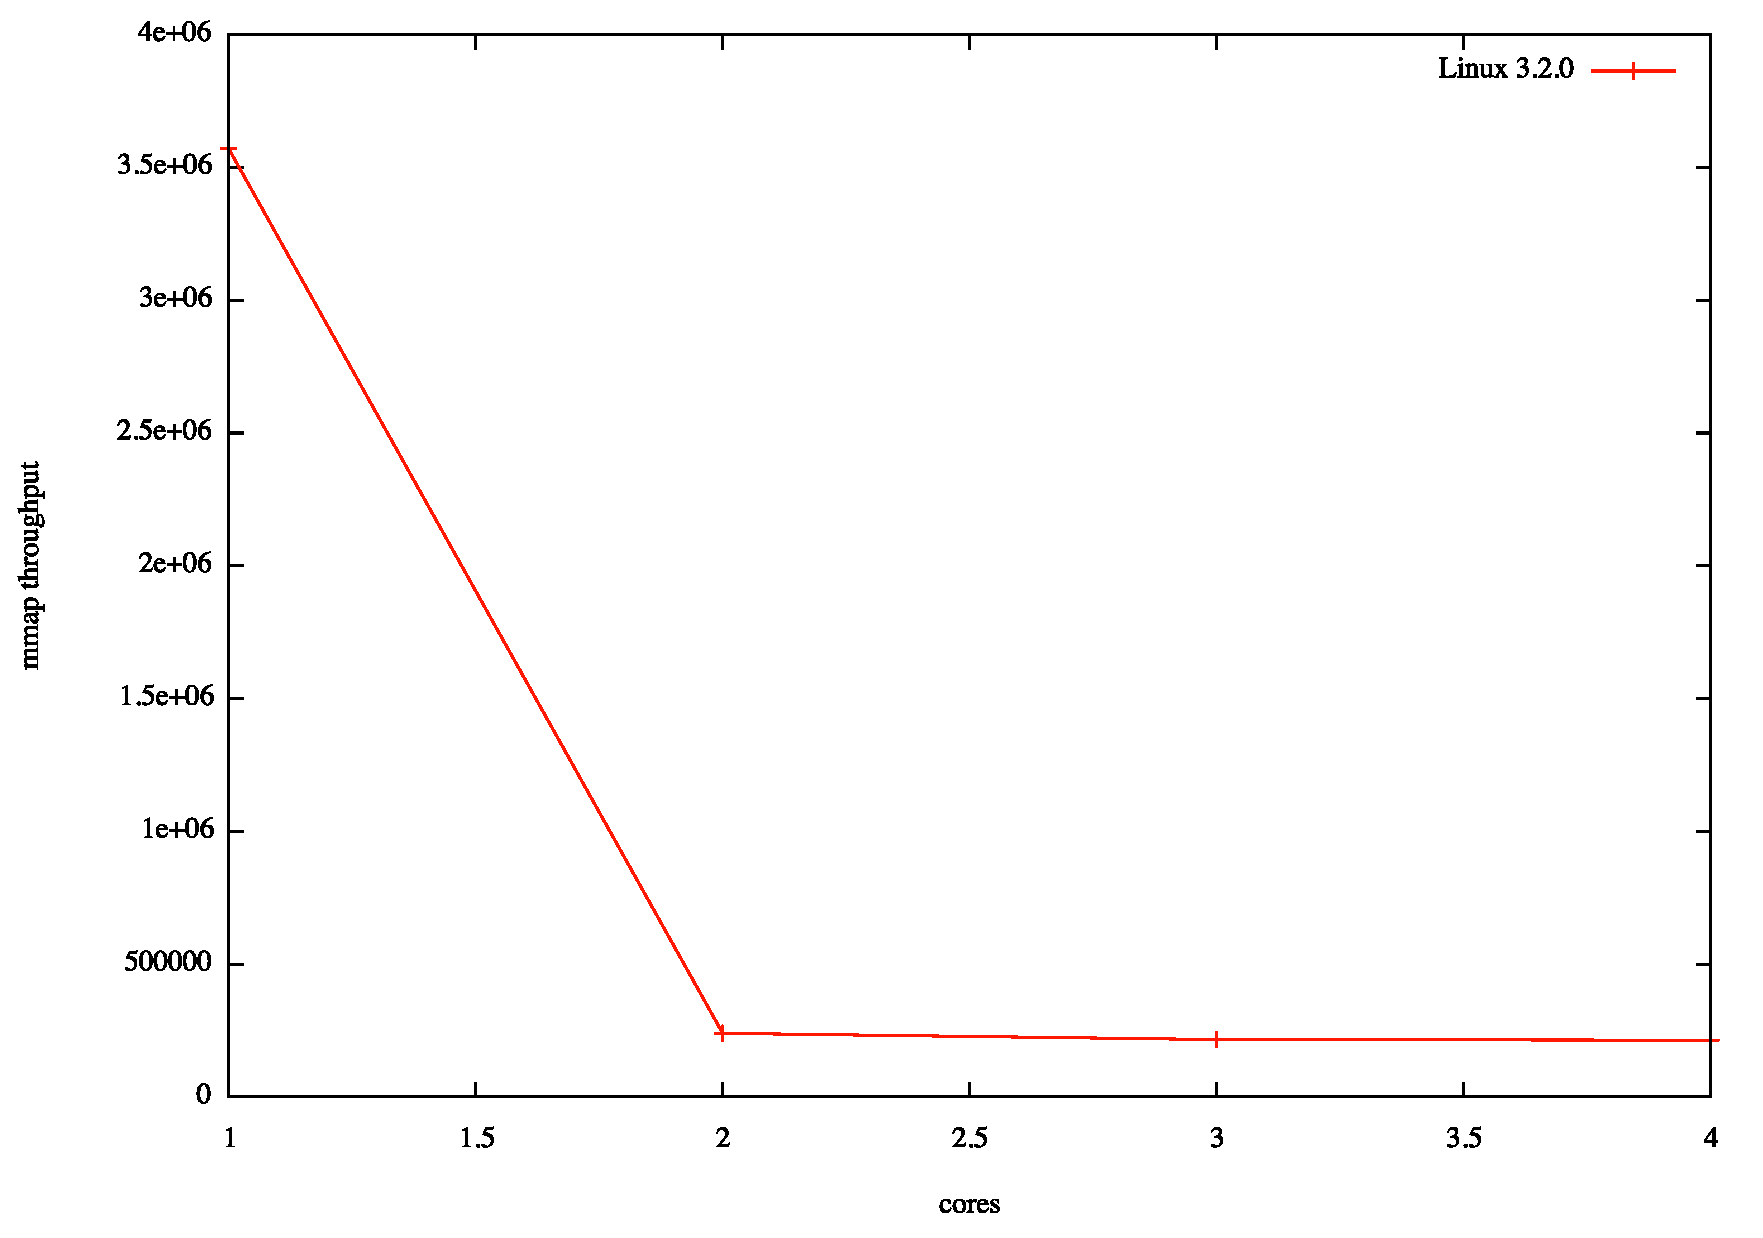
\includegraphics[width=0.8\textwidth]{figures/mmap_test.pdf}
\end{center}
\caption{多核系统mmap饱和测试}
\label{fig:mmap_test}
\end{figure}

\section{可交换性原理}

从上面的案例分析中我们可以知道,现有操作系统内核的部分子系统在多核硬件上表现不如人意。但是,在做出具体可扩展性优化之前,有必要充分论证这种优化的存在性。例如,根据Posix系统调用规范,open系统调用必须返回当前进程中最小的未被使用的文件描述符。如果严格遵循这种规范,open接口规范本身就无法做到并行可扩展,因为实现者必须串行化这些调用来获得最小的文件描述符。另一方面,对于mmap等调用,Posix标准并没有对匿名页返回地址做任何要求(用户指定除外),事实上,造成VM操作在Linux、FreeBSD上可扩展性问题的原因是他们使用了红黑树或伸展树来管理虚拟内存映射\cite{radixvm:eurosys13},这类数据结构需要一个大锁来保护其内部状态(如红黑树的内部节点)的一致性,即使VM操作涉及的是两个不相关的叶子节点。

为了解答可扩展性优化存在性问题,受到编译器优化技术的启发,有研究者提出了一种在系统接口(如Posix规范)中发现可扩展潜能的方法\cite{commuter:2013}。他们称之为``可交换性法则":只要两个操作的顺序可以交换,那么就可以用多核可扩展的方式实现这些操作。其中的原理是,如果两个操作可以交换(不影响操作结果,因此调用者无法分辨它们执行的顺序),那么他们就可以用不造成读-写冲突的方式实现。

根据这条规则,可以认为Syscall的可交换性在一定程度上等价于Syscall的多核可扩展性。
直观理解,当两个Syscall在一定条件下可交换,意味着他们没有数据相关性,通过某种实现可以避免多核CPU对二三级高速缓存的竞争(Cache
Contention),因此可以达到线性加速比(Perfect Scalability)。

理论上,为了发现系统调用可交换条件,需要遍历Syscall实现中的所有条件
分支,这可以用符号执行技术实现。但是真实Syscall实现过于复杂,
我们可以通过归纳Posix标准中对某个Syscall语义的要求,用简化
的模型(Model)描述此语义要求。

基于这条规律,我们提出了基于模型验证(model
checking)和符号执行的方法,求解Posix标准中系统调用的可交换条件。并尝试了使用KLEE\cite{Cadar:2008:KUA:1855741.1855756}解决问题符号执行的问题。

\section{简单建模例子 \pozhehao 引用计数}
本小结使用一个简单的例子,说明接口建模、交换性求解的整个过程。

引用计数器是跟踪对象生命周期的一种常用编程范式。在操作系统的关键数据结构(如共享物理页管理,VMA结构体,inode结构体等)中,都使用了引用计数器来跟踪这些对象的共享情况,当引用计数变为零时及时删除对象占用的内存,防止内存泄露。Linux等系统中,通常使用atomic\_t类型记录对象的引用计数:

\begin{lstlisting}
/* linux 3.9.2 include/linux/fs.h */
struct inode {                            
    /* ... */
    u64                     i_version;   
    atomic_t                i_count;     
};
\end{lstlisting}

正如本章开头所述,使用原子操作不利于操作系统的多核扩展。直观分析,若引用计数的值足够大,随便调换原子加减操作的次序并不会改变程序的运行结果,因此使用某种引用计数器计数,可以在多核上达到较好的可扩展性。
下面我们将对这种简单的引用计数器建模,使用符号执行技术发现其扩展性潜能,说明这种方法的可行性。

我们把引用计数器上的操作(API)抽象为个函数:
\begin{enumerate}
\item counter\_add
\item counter\_dec
\item counter\_iszero
\end{enumerate}

考虑计数器加一和减一操作,使用C编写对应的模型:

\begin{lstlisting}
void counter_add(struct state *counter)
{                                      
        counter->c ++;                 
}                                      
void counter_sub(struct state *counter)
{                                      
        if(counter->c>0)               
                counter->c --;         
        if(counter->c == 0)            
                counter->free = 1;     
} 
\end{lstlisting}


\section{虚拟内存管理子系统的建模}

近年来,随着SMT求解器,如STP、MathSAT、Z3的进步,为符号执行和模型验证方法提供了越来越强大的后端支持,使对操作系统等一类高复杂度软件的形式化验证成为了可能。事实上,在OSDI近年的会议上,已有多项针对OS中文件系统子系统的建模工作\cite{radixvm:eurosys13}\cite{Yang:2006:UMC:1189256.1189259},但他们的主要着眼点在使用模型验证和符号执行手段分析现有文件系统的Bug和错误上。
在文件系统方面,MIT的Commuter\cite{commuter:2013}的一个创新点是把符号执行与可交换性法相结合,提出了在Posix文件系统API规范中发掘多核可扩展机会的方法。

本毕设希望把Commuter的思路进一步扩展到OS的其他子系统,通过为操作系统虚拟内存管理、进程管理子系统进行建模,提供一种可以跨OS子系统分析操作系统接口多核可交换性/可扩展性的方法。

首先,我们认为对虚拟内存子系统系统调用建模发现潜在的可扩展性因素越来越有必要。正如文章\cite{radixvm:eurosys13}所说,在多核系统上OS的VM子系统对于VM密集型应用(如Java垃圾回收器)上已经成为了瓶颈,大大限制了多线程编程模型的多核可扩展性。通过建模发现Posix
VM API中可扩展性的潜能,以此为基础提出更好的Posix系统调用实现方式。

另一方面,我们认为对OS的虚拟内存管理系统/管理系统建模是一项比对文件系统建模更有挑战性的工作,有如下两个原因。

第一,文件系统主要以数据结构的更新逻辑为主,对open、read等系统调用建模时可以把底层硬件(如磁盘)抽象为数组。因此已有工作对文件系统相关系统调用都没有考虑硬件的影响。而对虚拟内存子系统建模时,必须考虑硬件缺页中断等硬件相关的影响。

第二,实际操作系统中,对虚拟内存和进程的管理设计大量共享可变数据结构(shared
mutable),如fork系统调用对物理页的写时复制(Copy-on-Write)策略,信号量的共享等。这种特性与Z3等SMT求解器以函数式语法描述程序约束条件的情况相对立,使得可交换性条件求解变得困难。

下面我们以操作系统中虚拟内存管理(Virtual Memory)子系统为例,介绍简化的Posix系统调用API接口和中断处理例程的建模方法。
在OS的虚拟内存管理子系统中,有两个最重要的系统调用:mmap和munmap。与文件系统建模不同的是,为了相对完整地描述虚拟内存子系统的行为,模型中还必须包括VM子系统对缺页异常(pagefault
handler)的处理例程。[XXX 如何扩展论述?]

对于内存管理子系统,我们把操作系统对程序的接口分成两类:
\begin{enumerate}
\item OS提供给用户态程序的系统调用接口,如mmap/mumap系列函数;
\item 用户程序访问硬件页表发生缺页中断时,操作系统根据虚拟地址区域的元数据(如Linux中的VMA结构体)填写缺失的硬件页表项。对于由软件填充TLB的体系结构,如MIPS,也可以通过软件模拟页表的方法实现类似功能。
\end{enumerate}

在编写操作系统的过程中,我们发现上述两类操作系统接口可以统一建模。由于在x86\_64(或其他大部分体系结构中)缺页异常属于同步异常\cite{intelsys},可以把读写缺页看做普通系统调用,通过添加如下两个虚拟系统调用对缺页进行建模:

\begin{verbatim}
void mem_write(pid, addr, value)
word mem_read(pid, addr)
\end{verbatim}

\subsection{系统调用建模}

\subsection{中断建模}

\section{基于模型的可交换性求解}

\subsection{基本算法}

\subsection{使用KLEE求解模型}
KLEE是基于LLVM
bytecode的符号执行引擎。KLEE已经被广泛地应用在文件系统建模,大型开源软件(如GNU
coreutils)漏洞查找\cite{Cadar:2008:KUA:1855741.1855756}等方面。KLEE中使用了一种简单的方法来避开指针和Heap对象约束求解的困难:记录指针可能引用的对象集合,在指针被dereference的时候,如果此指针可能指向N个对象,则fork出N个状态并进入调度队列,之后再继续进行符号执行。状态之间,KLEE使用写时复制(Copy-on-Write)的方式管理内存。有研究者对这种方法做扩展。


\subsection{进一步讨论}

实验中发现,KLEE并不能完全解决共享内存对象推导的问题。
Separation Logic是对Hoare
Logic的一种扩展,理论上可以用于对使用共享可变数据结构(如Heap上分配的对象)的命令式程序做推导[7]。考虑如下程序:

【XXX 多数sep logic论文使用reverse list。我们应该用OS中单向链表使用的例子】

形式上Separation Logic定义了Separating Conjuction运算符:P *
Q,表示程序的堆(Heap)可分割为两个独立的堆H1、H2,在H1上命题P成立,在H2上命题Q成立。直观上,通过Seperating
conjuction运算符和相关推理规则,简化了Heap上包含共享数据结构程序约束的描述。然而,文章[7]中并未给出Separation
logic的判定过程(decision
procedure),Z3等SMT求解器未支持此类逻辑的可满足性判定。但是,对于separation
logic的一些特殊情况,学界已经提出了相关的判定过程。例如,对于操作系统中的使用最频繁的链表结构,文章[9]提出了求解下面形式约束的算法,并在Z3
SMT求解器中实现:

[公式 XXX -> xxxxx]
其中XXX是xxx


\section{小结}
XXX TODO


\chapter{多核操作系统和相关性能测试工具的实现}
在上一章多核操作系统可扩展性理论的基础上,本章将介绍在清华uCore实验操作系统的基础上加入对最新NUMA的多核处理器的支持,并用数种多核可扩展的数据结构和算法改造其内核数据结构。

\section{AMD64多核NUMA架构硬件抽象层的实现}
本毕设在实验操作系统内核uCore的硬件抽象层基础上,加上了相对完整的x86\_64 NUMA多核架构支持。本内核已经在QEMU软件模拟器、KVM硬件虚拟化平台和Intel真实机器上测试通过。
\subsection{uCore硬件抽象层概述}

\subsection{ACPI支持}

\subsection{多核中断和IPI中断支持}

\section{多核操作系统基础设施实现}
\subsection{锁的实现}

\subsection{支持NUMA的物理页分配器}

\subsection{per-CPU变量实现}

\section{可扩展引用技术器的实现}

\section{基于QEMU的全系统性能采集工具}


%%% Local Variables:
%%% mode: latex
%%% TeX-master: t
%%% End:


\chapter{操作系统性能分析工具设计实现}

无论在程序的开发还是真实使用的过程中,发现和调试系统中出现的性能问题都是至关重要的。用户程序的性能优化迭代流程一般是这样的:
\begin{enumerate}
\item 使用性能采集工具(如GProf、Intel VTune等)对目标程序进行测试;
\item 通过测试结果,分析软件运行的关键路径,找到性能瓶颈;
\item 对关键路径上的数据结构和算法做优化,如效果不理想跳到1;
\item
当数据结构和算法都优化到最优状态后,进行体系结构相关优化,如Cache使用优化、使用内联汇编等。在此期间不断测试。
\end{enumerate}

从上述的软件优化流程可以看到,性能采集工具在优化过程中占有至关重要的作用。为此,开源软件界和工业界都开发了大量用户态性能测试工具,如开源的gprof和perf工具,和商用的Intel
VTune等。但是对于操作系统内核的有效性能分析工具却不多。虽然在Linux内核中集成了perf和ftrace性能分析子系统,这些工具都存在一些问题。最明显的是,它们与Linux内核耦合度太强,无法单独使用,因此无法对xv6、uCore等实验操作系统做性能测试。另外,这些工具运行在与内核相同的特权级别上,不能检测到系统内核的所有行为。为此,本毕设设计了基于QEMU的全系统性能采集工具QProf。本章将主要介绍QProf的工作原理。

\section{概述}
为了在模拟器中方便地寻找操作系统内核的瓶颈,本毕设这种方法结合了Qemu和gprof的两个开源软件,实现了一个全系统的Profiler
\pozhehao
QProf\footnote{https://github.com/chyh1990/qemu/tree/1.3-profiler},本系统具有以下特征:
\begin{itemize}
\item 通过模拟器,运行在比操作系统内核更高的级别上;
\item 使用了编译器的相关特性,不需对内核源代码做任何修改;
\item 生成与gprof兼容的测试报告,方便后期分析处理。
\end{itemize}

由于真实操作系统工作环境的复杂性,很难通过分析源代码等静态分析方法发现内核中的性能问题。
本全系统性能测试工具通过动态分析的方法,在内核运行过程中允许程序员方便地对操作系统内核的各个函数进行跟踪和计时。通过这些信息,可以较为容易地发现内核的运行的关键路径
(也正是内核代码的瓶颈所在),并发现潜在的性能问题。
真实应用上的测试结果第\ref{cha:test}章。

\section{QEMU模拟器架构分析}

QEMU\cite{Bellard:2005:QFP:1247360.1247401}是一个可移植的基于动态二进制翻译技术的硬件模拟器。QEMU可以模拟包括x86、PowerPC、ARM等多种CPU,并支持全系统硬件模拟,可以在这个模拟平台上运行Windows、Linux等多种操作系统。另外,在x86平台上,QEMU也支持KVM硬件虚拟化后端,大大提高了模拟器的执行性能。为了保证采样的正确性,现在QProf不支持KVM硬件虚拟化技术,但通过简单扩展可以方便实现。这里只对QEMU的软件动态二进制执行部分作讨论。

\begin{figure}
\centering
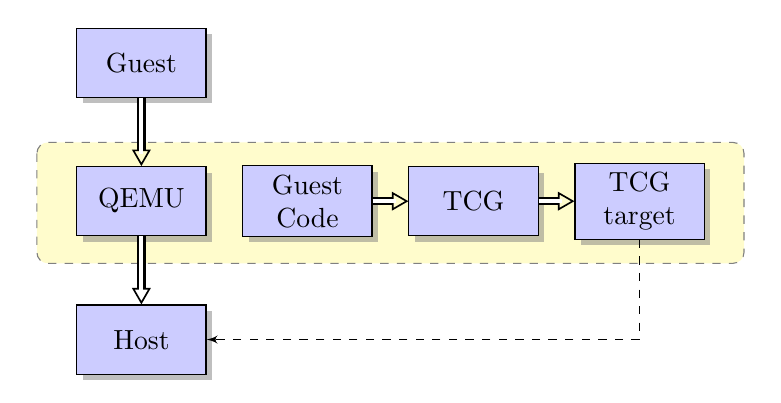
\begin{tikzpicture}

\tikzstyle{vecArrow} = [thick, decoration={markings,mark=at position
   1 with {\arrow[semithick]{open triangle 60}}},
   double distance=1.4pt, shorten >= 5.5pt,
   preaction = {decorate},
   postaction = {draw,line width=1.4pt, white,shorten >= 4.5pt}]

\tikzstyle{comp}=[draw, fill=blue!20, text width=4em, 
    text centered, minimum height=2.5em,drop shadow,node distance=5em]

\node[draw,comp] (a) {Guest};
\node[draw,comp,below of=a] (b) {QEMU};
\node[draw,comp,below of=b] (c) {Host};

\node[draw,comp,right of=b,node distance=6em] (gc) {Guest Code};
\node[draw,comp,right of=gc,node distance=6em] (tcg) {TCG};
\node[draw,comp,right of=tcg,node distance=6em] (target) {TCG target};

\draw[vecArrow] (a) to (b);
\draw[vecArrow] (b) to (c);

\draw[vecArrow] (gc) to (tcg);
\draw[vecArrow] (tcg) to (target);

\path [draw,-latex',dashed] (target) |- (c);

    \begin{pgfonlayer}{background}
        \path (b.west |- b.north)+(-0.5,0.3) node (a) {};
        \path (target.east |- target.south)+(+0.5,-0.3) node (c) {};

        \path[fill=yellow!20,rounded corners, draw=black!50, dashed]
            (a) rectangle (c);

    \end{pgfonlayer}


\end{tikzpicture}
\label{fig:qemu-arch}
\caption{QEMU模拟器系统架构}
\end{figure}

QEMU系统的架构见图\ref{fig:qemu-arch},其中的Tiny Code
Generator(TCG)是QEMU系统的核心,它把Guest的CPU指令翻译为QEMU内部的中间表示。对于普通指令,QEMU中有通用的指令实现代码。当遇到操作系统中的特权指令和涉及到协处理器、MMU操作等硬件相关指令时,QEMU将回调特定的Helper函数软件模拟硬件的行为。QProf使用这项特性,添加了一条AMD64
MSR控制寄存器的控制指令,实现被测试操作系统内核(Guest Code)对QEMU的回调。

另一方面,从QEMU的架构图中可以看出,QEMU工作在比被测试操作系统更高级的位置上。通过对QEMU进行修改,QProf可以准确地获得被测系统的全部状态。

\section{QProf工作原理}
	目前,对程序做性能测试的方法主要有两种:
	\begin{enumerate}
		\item {\heiti 插桩法}
			在程序编写、编译或链接(包括动态链接)的过程中,注入跟踪代码;
		\item {\heiti 采样法}
			系统中定时产生时钟中断时间,打断程序运行,采集当前程序计数器值(Program
			Counter)。通过采样点的分布,估计各个函数运行时间。
	\end{enumerate}

	QProf系统结合了上述两种方法对操作系统内核进行性能测试。它与传统用户态性能测试工具的主要区别是,QProf使用Qemu作为运行环境,可以跟踪CPU的底层状态。使用模拟器的跟踪操作系统内核性能情况的一个问题是,Qemu中使用软件模拟外设硬件的行为,如果操作系统的真正瓶颈在IO操作上(而非算法),则QProf难以直接发现真实的性能瓶颈。但是通过QProf采集的函数调用次数等其他信息,开发者可以分析和推测系统的问题所在。 QProf的主要原理如下所示:
	\begin{itemize}
		\item 编译内核时加入-pg参数,GCC会在所有
			函数的prolog中插入一个mcount函数调用,
			用于跟踪函数调用图(Call graph):
\begin{lstlisting}[language={[x86masm]Assembler}, caption=加入-pg编译参数后的函数序言]
<x2_cpu_init>:                                                 
	55                      push   %rbp                     
	48 89 e5                mov    %rsp,%rbp                
	48 83 ec 10             sub    $0x10,%rsp               
	e8 93 23 fb ff          callq  ffff80000022ce24 <mcount>
	48 89 7d f8             mov    %rdi,-0x8(%rbp)          
\end{lstlisting}

		\item 在内核中实现mcount函数,加入一条对Supervisor(QEMU)
			回调指令。在QProf中,使用如下汇编代表做回调:
\begin{lstlisting}[caption=QProf中mcount函数实现]
        movq    56(%rsp),%rsi
        /* Get frompc via the frame pointer.*/
        movq    8(%rbp),%rdi
        /* call the hypervisor */
        mov     $MAGIC_ECX, %ecx
        wrmsr
\end{lstlisting}
		\item 修改QEMU,对Supervisor的回调进行响应,生成调用图;
		\item QEMU中使用时钟信号定时采样,对内核做profile。
	\end{itemize}

\section{小结}



\chapter{系统测试与分析}
\label{cha:test}


\section{虚拟内存子系统模型求解结果}
\label{sec:vm-result}
对\ref{sec:vm-model}一节所述的虚拟内存子系统模型,使用相关算法进行交换性求解,生成的可交换测试用例数目如表\ref{tab:commute-stat}所示。

\begin{table}[ht]
  \centering
  \caption{可交换用例求解结果统计}
  \label{tab:commute-stat}
    \begin{tabular*}{0.6\linewidth}{ll|c}
      \toprule[1.5pt]
      {\heiti 系统接口1} & {\heiti 系统接口2} & {\heiti 可交换测试用例数} \\\midrule[1pt]
mmap & mmap & 36             \\
mmap & munmap & 18           \\
mmap & pgfault\_read & 24     \\
mmap & pgfault\_write & 24    \\
munmap & munmap & 9          \\
munmap & pgfault\_read & 12   \\
munmap & pgfault\_write & 12  \\
      \bottomrule[1.5pt]
    \end{tabular*}
\end{table}

分析求解结果可以发现,造成这组系统调用不可交换的原因主要是涉及重叠虚拟地址的操作,如先后用不同参数mmap同一个虚拟地址。根据``可交换性原理'',对于不涉及重叠区域的虚拟地址映射操作,存在一种多核可扩展的mmap/munmap实现。事实上,学术界已经提出了RCU平衡树\cite{Clements:2012:SAS:2189750.2150998}和RadixVM\cite{radixvm:eurosys13}等数据结构优化虚拟内存子系统的多核可扩展性。


\section{uCore系统启动测试}
uCore多核操作系统内核可以运行在QEMU软件模拟器、KVM硬件虚拟化平台和Intel真实机器。
图\ref{fig:ucore-init}和图\ref{fig:ucore-normal}是uCore在此KVM硬件虚拟化平台
(两个NUMA节点,8个CPU核)上的运行情况。

\begin{figure}[ht]
\begin{minipage}{0.48\textwidth}
  \centering
  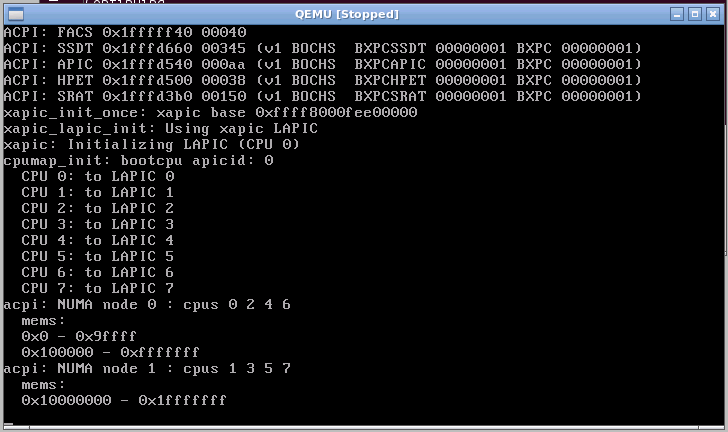
\includegraphics[width=\textwidth]{figures/ucore_init.png}
  \caption{KVM中启动情况}
  \label{fig:ucore-init}
\end{minipage}\hfill
\begin{minipage}{0.48\textwidth}
  \centering
  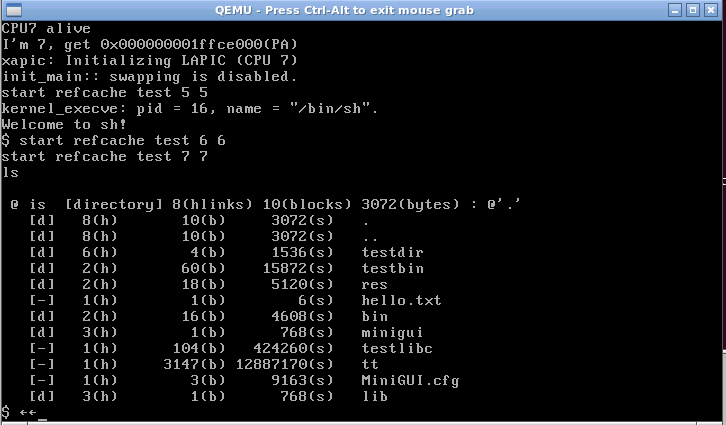
\includegraphics[width=\textwidth]{figures/ucore_normal.png}
  \caption{多核系统上正常运行}
  \label{fig:ucore-normal}
\end{minipage}
\end{figure}

在图\ref{fig:ucore-init}中可以看出,uCore在KVM中正确读取硬件固件中的ACPI信息表,并检测出NUMA节点上的CPU和内存信息。BSP初始化内核完成后,唤醒余下AP,最后把控制交给用户态程序,系统运行正常。

为了方便地在AMD64硬件平台上调试,本毕设在uCore中加入了Grub2引导系统支持,可以方便地使用PXE和Grub2无盘网络启动uCore。下面的为uCore在一台Intel
Core
4核机器上的启动日志,可以发现真实机器上可能缺少某些ACPI表项,因此在操作系统的初始化过程中必须为这些配置信息设定适当的默认值,确保系统正常启动。

{\tiny
	\begin{Verbatim}[frame=single]
(THU.CST) os is loading ...

Multiboot dectected: param 0x10000
mbmod: 0 0x29e000 0x69e000
acpitables_init()
ACPI: RSDP 0xf6d00 00014 (v0 GBT   )
ACPI: RSDT 0x7dce3040 0003c (v1 GBT    GBTUACPI 42302e31 GBTU 01010101)
ACPI: FACP 0x7dce30c0 00074 (v1 GBT    GBTUACPI 42302e31 GBTU 01010101)
ACPI: DSDT 0x7dce3180 042d4 (v1 GBT    GBTUACPI 00001000 MSFT 0100000c)
ACPI: FACS 0x7dce0000 00040
ACPI: HPET 0x7dce75c0 00038 (v1 GBT    GBTUACPI 42302e31 GBTU 00000098)
ACPI: MCFG 0x7dce7640 0003c (v1 GBT    GBTUACPI 42302e31 GBTU 01010101)
ACPI: TAMG 0x7dce7680 0644a (v1 GBT    GBT   B0 5455312e BG?? 00020101)
ACPI: APIC 0x7dce74c0 00084 (v1 GBT    GBTUACPI 42302e31 GBTU 01010101)
ACPI: SSDT 0x7dcee3f0 003ab (v1  PmRef    CpuPm 00003000 INTL 20040311)
xapic_init_once: xapic base 0xffff8000fee00000
xapic_lapic_init: Using xapic LAPIC
xapic: Initializing LAPIC (CPU 0)
cpumap_init: bootcpu apicid: 0
  CPU 0: to LAPIC 0
  CPU 1: to LAPIC 1
  CPU 2: to LAPIC 3
  CPU 3: to LAPIC 2
numa_init: SRAT not found! Assuming one NUMA node
memory management: buddy_pmm_manager
e820map: size, begin, end, type
----------------------------------------
  memory: 000000000009f800, [0000000000000000, 000000000009f7ff], Usable.
  memory: 0000000000000800, [000000000009f800, 000000000009ffff], Reserved.
  memory: 0000000000010000, [00000000000f0000, 00000000000fffff], Reserved.
  memory: 000000007dbe0000, [0000000000100000, 000000007dcdffff], Usable.
  memory: 0000000000003000, [000000007dce0000, 000000007dce2fff], ACPI NVS memory.
  memory: 000000000000d000, [000000007dce3000, 000000007dceffff], ACPI reclaimable memory.
  memory: 0000000000010000, [000000007dcf0000, 000000007dcfffff], Reserved.
  memory: 0000000010000000, [00000000d0000000, 00000000dfffffff], Reserved.
  memory: 0000000001400000, [00000000fec00000, 00000000ffffffff], Reserved.
--------Total Usable Phy Mem Size 2012 MB-----------
numa_mem_zone 0: 0x0000000002612000 - 0x000000007b6cdfff, 1974MB
	\end{Verbatim}
}

编写同时支持真实机器和模拟器的uCore内核是重要的,因为两种运行环境都有各自的优势和不足。

\section{多核支持测试}
为了测试多核uCore对系统CPU核的使用情况,本毕设编写了一个简单的并行矩阵乘法用户态程序matrix。默认情况下,此程序将使用系统中所有可用CPU内核经行计算\footnote{测试环境:Intel
i5 3.0GHz, 4核机器}。表\ref{tab:mp-matrix}是本程序在不同CPU核数上运行时间的测试结果,可见运行时间大致与核数成反比关系,与理论分析一致。

\begin{table}[ht]
  \centering
  \caption{uCore多核测试}
  \label{tab:mp-matrix}
    \begin{tabular*}{0.6\linewidth}{c|ll}
      \toprule[1.5pt]
      {\heiti CPU核数} & {\heiti 用时/秒} \\\midrule[1pt]
      1 & 13.70  \\
      2 & 7.40  \\
      4 & 4.00   \\
      \bottomrule[1.5pt]
    \end{tabular*}
\end{table}



\section{可扩展引用计数器测试与分析}
在四核机器上,使用7个内核线程(另外一个主线程控制测试)对引用计数器进行测试。原子操作指令和Cache竞争是造成引用计数器可扩展性问题的根源,表\ref{tab:refcache-stat}比较了使用普通原子操作和Refcache对内存总线加锁的次数。

\begin{table}[ht]
  \centering
  \caption[Refcache性能对比]{普通原子操作和Refcache对内存总线加锁的次数对比($flush\_time =
  10ms$)}
  \label{tab:refcache-stat}
    \begin{tabular*}{0.6\linewidth}{c|ll}
      \toprule[1.5pt]
      {\heiti $dec/inc$次数} & {\heiti Atomic} & {\heiti Refcache}  \\\midrule[1pt]
	30  & 30   & 8	 \\
	44  & 44   & 8   \\
	58  & 58   & 10  \\
	72  & 72   & 12  \\
	86  & 86   & 14  \\
	100  & 100   & 16  \\
	114 & 114  & 18  \\
	128 & 128  & 20  \\
	142 & 142  & 20  \\
	226 & 226  & 20  \\
	240 & 240  & 22  \\
	254 & 254  & 22  \\
	268 & 268  & 22  \\
      \bottomrule[1.5pt]
    \end{tabular*}
\end{table}

\begin{figure}[ht]
\begin{minipage}{0.48\textwidth}
  \centering
  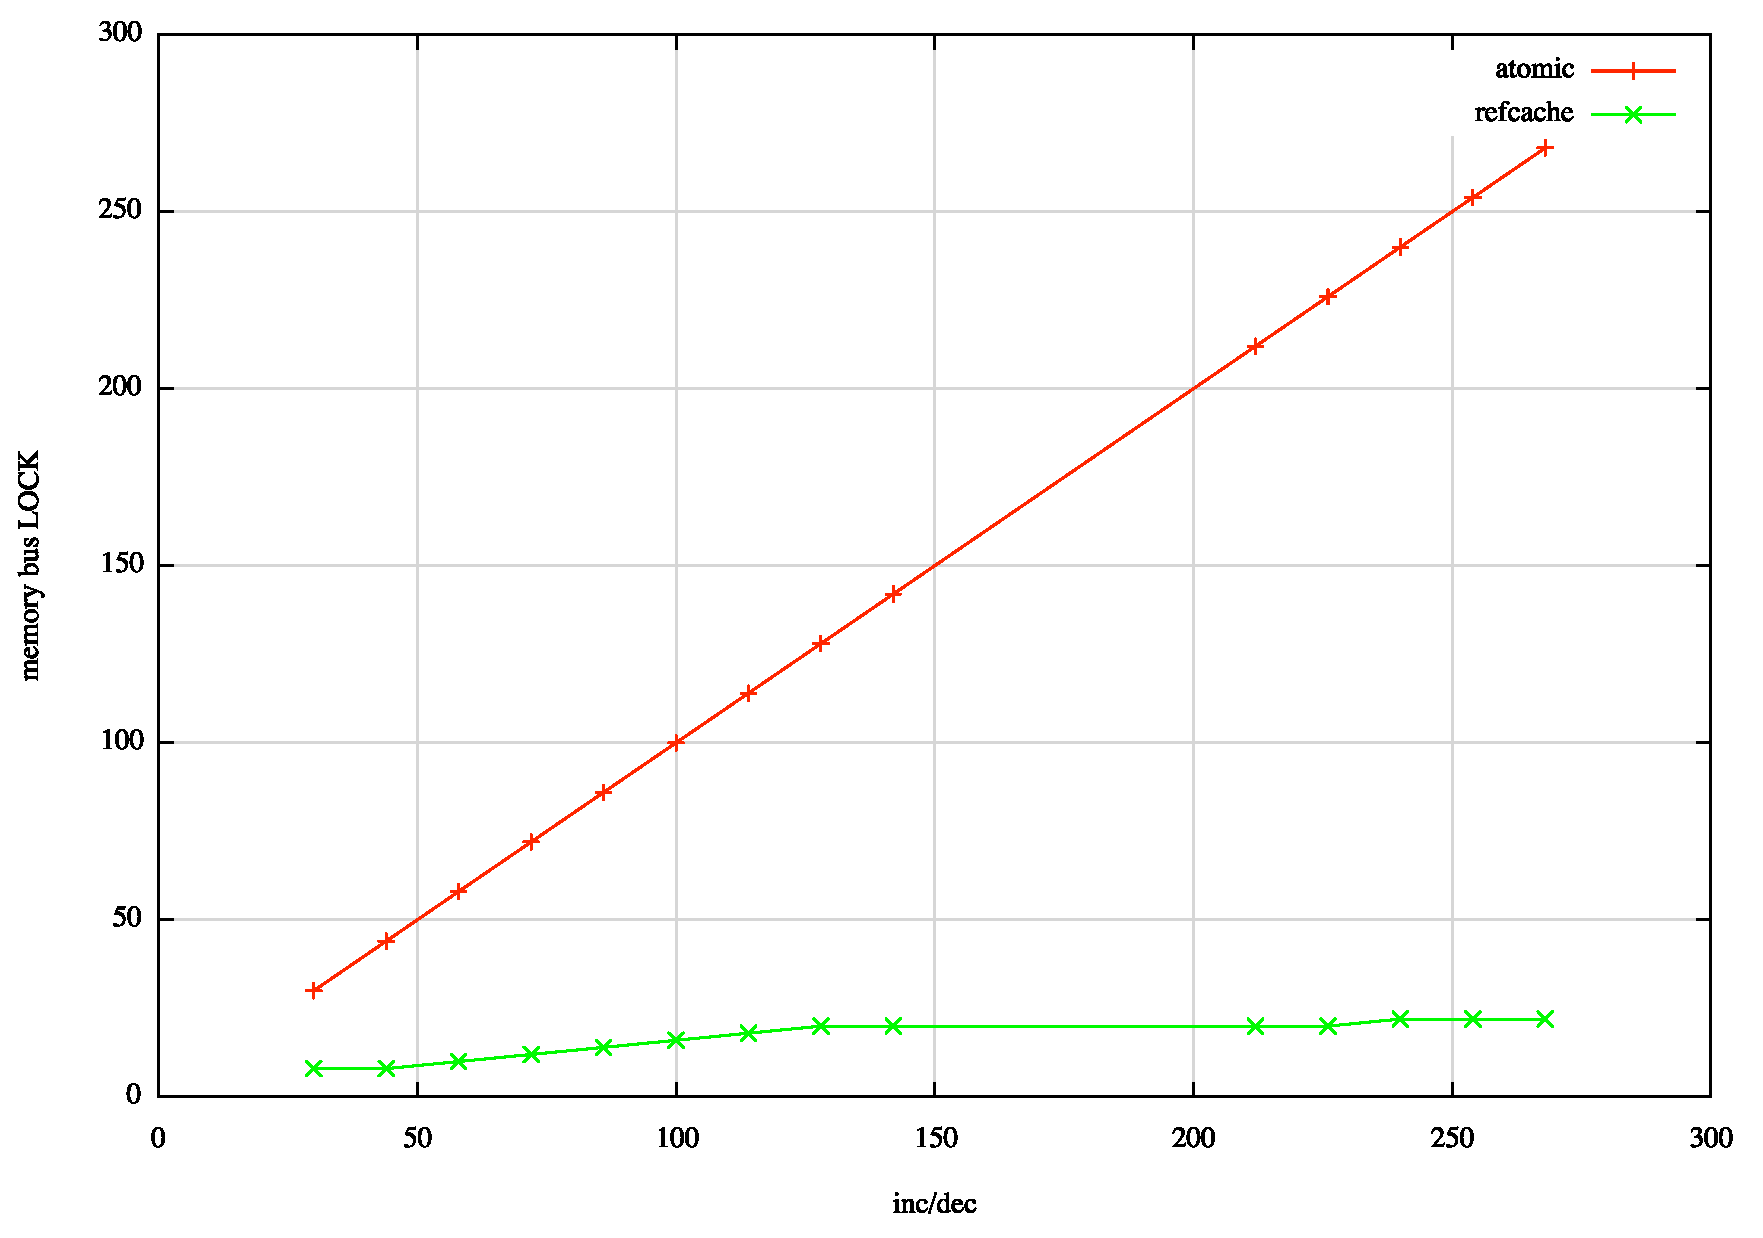
\includegraphics[width=\textwidth]{figures/refcache1.pdf}
\end{minipage}\hfill
\begin{minipage}{0.48\textwidth}
  \centering
  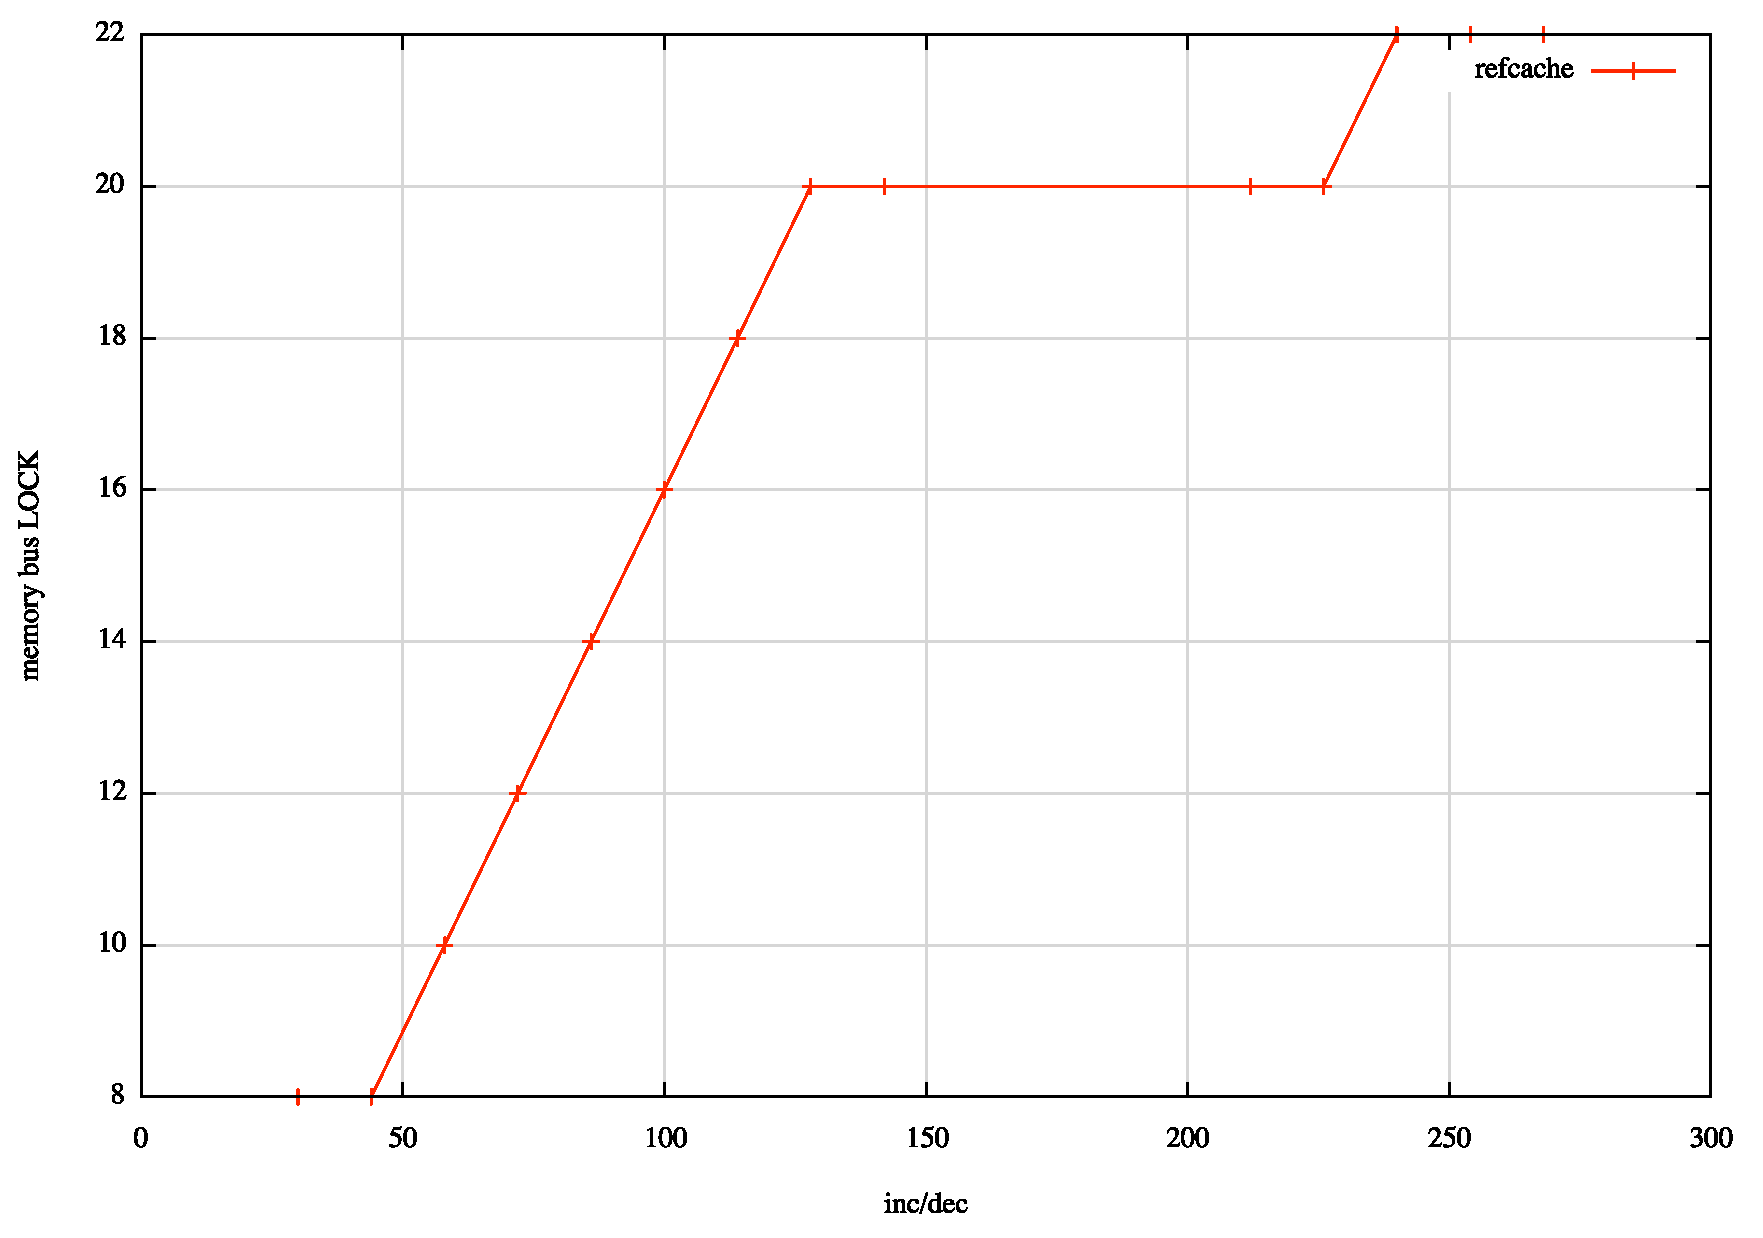
\includegraphics[width=\textwidth]{figures/refcache2.pdf}
\end{minipage}
\caption{Refcache性能对比}
\label{fig:rc-cmp}
\end{figure}

由图\ref{fig:rc-cmp}测试结果可以看出,Refcache的全局同步次数成阶梯状方便,这是因为Refcache在多数情况下只在时钟中断到来是发起全局同步操作,并判断对象引用次数是否为0。Refcache使用CPU本地缓存吸收了大量inc和dec操作,更新全局计数器的次数大大减少。因而Refcache比使用一般原子操作在多核系统上有更好的可扩展性表现。

\section{QProf测试}
为了使用本测试系统,必须使用修改过的Qemu软件模拟器运行内核:
\begin{enumerate}
	\item 首先,在编译内核时加上-pg参数;
	\item
		使用修改过的Qemu,使用下面的命令行参数运行uCore或其他操作系统内核:
		\begin{lstlisting}[language=sh]
qemu-system-x86_64 -no-kvm -m 512 -hda \
obj/kernel.img -profileelf kernel-amd64.elf
\end{lstlisting}

		并在操作系统中运行微测试应用程序;
	\item
		内核运行结束,Qemu退出后将生成kgmon.out文件,可以使用标准的gprof工具解析:
		\begin{lstlisting}[language=sh]
gprof obj/kernel/kernel-amd64.elf kgmon.out
\end{lstlisting}

\end{enumerate}

	例如,本毕设使用QProf寻找uCore中readdir系统调用运行缓慢的原因。在uCore上多次运行使用
	\emph{ls}命令列出目录,并使用QProf记录系统性能信息:
	{\tiny
	\begin{Verbatim}[frame=single]
Flat profile:

Each sample counts as 0.01 seconds.
  %   cumulative   self              self     total
 time   seconds   seconds    calls  ms/call  ms/call  name
 25.62      0.52     0.52     8654     0.06     0.06  ide_wait_ready
  8.87      0.70     0.18      960     0.19     0.75  ide_read_secs
  8.37      0.87     0.17                             do_halt
  4.43      0.96     0.09     1195     0.08     0.08  memmove
  4.19      1.05     0.09   135219     0.00     0.00  get_pte
  2.96      1.11     0.06     7908     0.01     0.01  serial_putc_sub
  2.71      1.16     0.06   135268     0.00     0.00  get_pmd
  1.97      1.20     0.04   433010     0.00     0.00  ptep_present
  1.97      1.24     0.04      673     0.06     0.06  memset
	\end{Verbatim}
	}

	通过QProf也可以获得内核的函数调用图:

	{\tiny
	\begin{Verbatim}[frame=single]
granularity: each sample hit covers 2 byte(s) for 0.49% of 2.03 seconds

index % time    self  children    called     name
                0.00    1.25    4377/4377        __alltraps [2]
[1]     61.4    0.00    1.25    4377         trap [1]
                0.00    1.24    4377/4377        trap_dispatch [3]
                0.01    0.00   26695/26889       mycpu [157]
                0.00    0.00    8746/8755        trap_in_kernel [365]
                0.00    0.00    4362/4362        kern_enter [376]
                0.00    0.00    4355/4362        kern_leave [377]
                0.00    0.00    4278/4285        may_killed [379]
                0.00    0.00      79/117         schedule [429]
	\end{Verbatim}
	}

	通过上述数据,开发者可以发现ide\_wait\_ready和ide\_read\_secs运行次数非常多,
两个函数耗时约占系统运行总时间的35\%。进一步分析可以发现,uCore虚拟文件系统(Virtual
Filesystem,VFS)中没有实现类似Linux的Page
Cache机制和IO调度机制,在执行ls命令时,内核需要多次读取磁盘上不连续的扇区,导致磁盘IO
性能问题。



\chapter{总结}

本毕设完成了在AMD64多核平台下,针对操作系统上的多核可扩展性问题,进行了理论上的分析,并完成了uCore多核支持和相应的性能测试工具。具体来说,本毕设所做的工作如下:

\begin{itemize}
	\item
	调研了研究界和工业界在操作系统多核可扩展性上所做的工作,为本系统的实现奠定了基础
	\item
	介绍了对操作系统虚拟内存子系统接口(包括系统调用和硬件中断)建模的方法,并提出了使用KLEE对接口模型做可交换性求解的方法
	\item 在实验操作系统uCore上实现了多核硬件无关层模型和AMD64 NUMA多核硬件平台的支持
	\item
	在上一点实现的硬件无关层上,实现了无锁堆栈、可扩展percpu变量、Refcache引用计数器和NUMA物理页分配器等多核可扩展操作系统基础设施
	\item 提出了一种新的基于QEMU模拟器的性能测试工具QProf
\end{itemize}

本毕设所提出的用KLEE求解系统接口可交换性的方法具有一定的研究价值。另一方面,本毕设在uCore上实现的多核架构基础设施,为以后的多核操作系统可扩展性研究和教学奠定了基础。由于本毕设设计的uCore
AMD64平台支持不但可以在真实机器上运行,还可以在QEMU和KVM模拟器上运行,大大降低内核调试的难度。最后,本毕设提出的QProf性能测试工具,提供了一种简便的全系统性能测试手段,具有较大的应用价值。

从另一方面看,本毕设的操作系统建模方法和uCore多核操作系统还有进一步完善的空间。首先,本毕设设计的虚拟内存系统模型并没有考虑文件映射内存页和进程见共享内存等情况。为了求解这些情况下的系统接口的交换性,必须对操作系统内核中其他子系统进行建模。其次,尽管本毕设实现了多核实验性操作系统原型uCore
AMD64,还需要大量的工作才能使其支持Metis\cite{linux:osdi10}等复杂应用。




%%% 其它部分
\backmatter

% 本科生要这几个索引,研究生不要。选择性留下。
\makeatletter
\ifthu@bachelor
  % 插图索引
  \listoffigures
  % 表格索引
  \listoftables
  % 公式索引
  \listofequations
\fi
\makeatother


% 参考文献
\bibliographystyle{thubib}
\bibliography{ref/refs}

\chapter*{发表论文情况}
 \begin{enumerate}[{[}1{]}]
\item 第九届和谐人机环境联合学术会议(HHME2013),已投
  \end{enumerate}

% 致谢
%%% Local Variables:
%%% mode: latex
%%% TeX-master: "../main"
%%% End:

\begin{ack}
  由衷感谢导师陈渝副教授对本人的细致指导。陈渝老师以丰富的研究经验和扎实的理论基础为我指明了研究方向,并在论文撰写期间提出
了诸多宝贵意见。另外,向勇老师在毕设过程中也给予了我悉心指导和鼓励。在此向两位老师表示诚挚的感谢!
同时感谢美国麻省理工学院PDOS研究组在实验操作系统设计和编写上给予的宝贵帮助!
\end{ack}


% 附录
\begin{appendix}
%%% Local Variables: 
%%% mode: latex
%%% TeX-master: "../main"
%%% End: 

\chapter{外文资料书面翻译}

\begin{center}
RadixVM: Scalable address spaces for multithreaded applications
\end{center}

\section{摘要}

RadixVM是一个新的虚拟内存管理系统(Virtual
Memory)的设计,使得在硬件保证Cache一致性的多核计算机系统上,多线程程序共享地址空间操作可以完全并发地经行。现在,大多数操作系统中mmap和munmap都是串行经行,这迫使程序员把他们的多线程程序分割成多个多进程程序,或者保留分配后的内存以避免返回这些内存到操作系统造成的额外性能损耗。RadixVM系统通过保证对不重叠虚拟地址空间操作的完全可扩展性,把开发者从这些繁杂的优化任务中解脱出来。

RadixVM结合了如下三种新技术:1、通过基数树(radix
tree)而不是平衡树来管理VMA结构,避免不必要的Cache
line冲突;2,使用新的,节省内存的分布式引用计数技术;3,使用新的远程TLB无效化(TLB
shootdown)策略,避免不必要的核间通信。
我们在80核的机器上经行了实验,发现RadixVM系统在非重叠虚拟内存区域中达到了完美可扩展。换言之,如果多个线程并行地地经行mmap和munmap系统调用,这些调用可以完全独立运行,并且不会带来Cache一致性协议造成的多核通讯流量。


\section{介绍}
在多核处理器系统上,多线程程序的性能瓶颈可能会发生操作系统中虚拟内存子系统的锁竞争上。虚拟内存子系统为了保证数据结构的复杂一致性,多数被广泛使用的内核,例如Linux和FreeBSD,都对每个共享地址空间(进程的VMA结构)加上了一把大锁。
近年来的研究已经发现了一些让缺页处理程序(page fault
handler)和mmap/munmap系统调用(用于从操作系统分配和释放内存)并行执行的方法。但是,如果mmap和munmap操作涉及的虚拟地址空间不重叠(例如内存分配和释放的场景下),理论上这些系统调用可以完美地并行化。这篇文章主要贡献就是在虚拟内存子系统中达到了这个目标。

一个传统的虚拟内存子系统支持三种关键操作:mmap用于向进程的VMA中加入一个区域,munmap用于删除一段区域,pagefault用于在缺页时根据VMA向硬件页表中插入记录,并在必要时分配物理页。这篇文章主要面向这样的一类用户程序:使用多线程模型在同一个VMA中频繁地并发发起上述几种操作。多线程内存访问频繁的程序最匹配这种模式:mmap、munmap和相关变形通常是高性能内存分配器和垃圾回收器实现的核心调用。频繁对文件经行映射和删除映射的用户程序也为操作系统内核的内存子系统产生压力,适合本文的应用场景。

因为操作系统及时对非重叠内存区域也会串行化mmap和munmap的调用,这类应用程序的瓶颈很容易发生在操作系统内核中。作为结果,用户程序开发者通常使用一些技巧绕开虚拟内存子系统造成的瓶颈。多线程内存分配器提供了很多这样的技巧:它们通常为每个线程向操作系统申请一大块内存,或延后munmap调用,或根本不返回内存到操作系统。有的程序提供一个内核可加载模块实现自定义的VM操作以提高分配器的性能。这些技巧都有各自的限制。

很多时候使用这些技巧已经足够避开OS内部VM的瓶颈,但通常有若干缺点。例如,一个Google工程师告诉我们,由于munmap的多核扩展性问题Google使用的内存分配器不精确地向OS返回内存。这样造成用户程序在退出前占用数GB的内存。这会延迟其他程序的启动甚至造成服务器使用效率低。其他公司的工程师也向我们反映相似问题。

随着系统CPU核数的增加,我们相信这些技巧会越来越复杂,并且缺点会越来越明显。
因此,我们的文章着眼与解决VM可扩展性问题的根源。我们的文章将提出一种新的虚拟内存管理子系统设计,它只在VM操作包含重叠区域时才会出现竞争现象。这保证了两个线程在操作不同的VM区域时,操作系统不会造成性能瓶颈,因此上述的技巧也不需要。在这种情况下,虚拟内存操作随着核心数线性扩展。如果应用程序使用多线程操作同一VM区域,两个线程之间共享竞争是不可避免的,但本系统可以限制使用的共享内存区域CPU核心。

为了达到并发的mmap/munmap操作,在虚拟内存系统的设计过程中存在几个挑战。
第一,虚拟内存系统不同部分之间维护着十分复杂的数据结构。例如,当munmap一个内存区域时,内核需要保证在回收物理页前删除硬件页表中的记录。否则,同一进程的其他线程可能会访问到其他进程的内存页面。为了保证内核正确实现这些操作的语义,内核必须保证一系列操作的顺序,这可能会在多核系统上造成性能瓶颈。
第二、即使是单个被多核竞争的Cache
line也可能成为多核系统的性能瓶颈。我们的一个原始设计是使用无锁可并发跳表(skip
list),但是跳表的内部节点会造成Cache Line竞争,限制了它的多核可扩展性。
第三、TLB无效化。为了保证没有CPU核心缓存过期的地址映射,CPU必须通过核间通信保证TLB一致性。第四、很多VM设计使用较为直接的方法避免VM锁的竞争,但是带来很大的内存代价。

本文提出了一个称为RadixVM的新设计。RadixVM使用三个不同的组件来使VM操作对非重叠内存区域具有完美可扩展性。
第一、我们设计了radix tree数据结构来记录虚拟内存映射。
第二、使用新的可扩展性引用计数来对共享物理页进行计数。
第三、但一个页面被unmap时,我们避免不必要的TLB无效化。
这三项措施使得我们的RadixVM系统具有极好的多核可扩展性。

我们在一个新的研究用内核xv6上实现了RadixVM,因为对Linux的虚拟内存系统做修改需要很大的工作量(Linux的VM子系统与其他子系统具有很强耦合性)。我们在80核的机器上测试了我们的系统,使用了Mosbench中的多线程的MapReduce库。单元测试测试显示我们的RadixVM系统达到了很好的可扩展性。

在xv6上,而不是Linux上实现RadixVM的一个缺点是xv6无法运行复杂的大型应用,如Oracle的Java虚拟机中的垃圾回收器。另一方面,RadixVM面临着一个蛋鸡问题:很多VM受限应用已经使用一些技巧来避免传统VM系统的扩展性问题。作为结果,我们的实验使用微型测例来做测试。


\section{设计}
实现不同进程中的可扩展的VM操作很容易,因为每个进程涉及到不同的VMA结构。RadixVM的设计是新颖的,因为它允许同一进程的多个线程同时执行mmap/munmap或缺页的操作(对非重叠的内存区域)。也就是说,如果在同一进程中的n个线程分配内存,这些mmaps是完美可扩展的(每次操作花费同样的时间,不论n多大)。同样,如果一个线程在一个CPU核上分配内存,同一进程中的另一个线程在另一CPU核操作系统返回不同的内存区域,那么这些操作不减慢或干扰对方的任何的mmap操作。最后,如果一个CPU核心上正在运行访问缺页处理例程,而其他CPU核进行VM操作(不包括pagefault),RadixVM也能达到完美可扩展性。另一方面,如果使用mmap和munmap对重叠内存区域进行操作,或者一个线程在mmaped或munmaped的页面上发生缺页,RadixVM将串行化那些操作。这种设计的可扩展性,可以容易地被应用程序开发人员了解和利用:应用程序只需要简单地避免对重叠内存区域并发操作。

为了在现代多核计算机实现完美的可扩展性,RadixVM努力确保CPU核不发生任何Cache
Line竞争。在现代的Cache一致性的硬件上,任何争用的Cache
Line的行为都可能是一个造成可扩展性问题的风险,因为频繁写入的多核共享的Cache
Line时,其他CPU核必须重新读取Cache内容,这种访问通常在Cache
Line的主节点上被串行化。

本节介绍RadixVM如何达到非重叠区域的VM操作的完美可扩展。首先,我们提出三个关键数据结构,然后介绍如何使用这些数据结构来实现标准的VM操作。

\subsection{使用Refcache来进行引用计数}
引用计数在很多操作系统中都非常关键,对RadixVM也一样,因为两个VM区域可能共享相同的物理页。例如Fork新进程时,RadixVM必须通过引用计数来计算需要释放的物理页。要做到这一点。RadixVM引用计数每一个物理页。但简单的引用计数器可能会导致可扩展性问题。因为多个线程将在计数变量上竞争。同样,RadixVM需要使用引用计数对Radix
tree的节点确定它们何时为空。

此的部分介绍Refcache,一种新型的引用计数方案。RadixVM使用Refcache来跟踪和回收的物理内存页面和基数树节点。Refcache实现高效空间的、懒惰的、可扩展的引用计数
--
每个CPU核有一个引用变化量缓存。Refcache针对可以容忍一定程度的延迟,且资源回收、递增和递减操作经常会发生在相同的核心的应用(例如,在同一个线程在发生pagefault的内存区域也unmap映射区域)。

Refcache与现有可扩展性的引用计数机制相比,需要的空间和需要引用计数的对象的数目加上CPU核心数,而不是其积成正比,每个CPU核心可以通过调整Delta的大小来在空间和可扩展性上做平衡。这点非常重要的,当一个大型的多核VM子系统需要在大CPU核数上跟踪每一个物理页,传统的可扩展的引用计数器将需要超过物理内存的一半来跟踪余下的物理内存。

Refcache缓存递增和递减操作并批量处理,这减少Cache
Line的竞争,同时提供一个可调的时间控制当其引用计数下降到零后,对象被垃圾回收的延迟。但一个对象只在单核上修改不会发生Cache
Line竞争,而Refcache自身只需要以恒定速率修改Cache Line来维护全局状态。

\textbf{基本Refcache}
在Refcache中,每个引用计数的对象都包含一个全局计数器,每个核维护一个本地固定大小的缓存,用来保存本CPU核上的计数增量。计数的增减只对本地增量Cache进行修改,本地CPU
Cache定时被刷新到对象的全局引用计数中。真正的计数值一般是未知的,但我们假设,一旦它下降到零,它会保持为零(在弱引用的情况下,我们将在后面讨论)。
Refcache依赖于真实计数为零后一直稳定到零的性质。

\subsection{Radix tree}
本质上,一个地址空间是一个从虚拟地址到元数据和物理内存的映射。为了完美地实现可扩展的非重叠的地址空间操作,RadixVM需要一个数据结构,可以跟踪此映射和支持mmaping和munmaping,同时避免不相交的虚拟内存区域上的VM操作之间的争。

避免竞争的一个方法是避免共享。例如,开发者定义把地址空间静态地分配到各个CPU核上,每个核各自管理自己的地址空间。这种方法保证了非重叠内存区域上的元数据访问不会发生冲突。这种方法的缺点在于它复杂化了数据共享,并且需要应用开发者感知这种划分。一个更好的解决方法是使用一些共享的数据结构,它允许多个线程对称地管理共享内存地址区域,这也是现在所有VM子系统的做法。

特别地,支持无锁操作的数据结构,如Bonsai树的读操作似乎是有可行的,因为它避免了由于锁导致的Cache
Line竞争。然而,无锁定操作,并不意味着没有Cache
Line竞争。例如,对于插入和查询操作,无锁的并发Skip
list可能会导致在涉及不同的节点上查找和插入键出现Cache
Line竞争,因为保持$O(\log
N)$查找节点的数据复杂度。插入操作必须修改内部节点。正如我们将在后面所述,该读写共享造成严重的扩展性问题,因为更多的CPU核需要重写读取被修改的Cache
Line,及时这些修改与它自身无关。

任何平衡树或类似的数据结构受到这种的Cache
Line竞争影响。一种解决方案(完全不切实际)是代表用一个线性数组来存储进程的虚拟内存映射的元数据,
对每个虚拟页面,单独在一个大线性数组上进行虚拟页号索引。在这种线性表示下,mmap/munmap,缺页的无锁地进行。
在非重叠的内存区的VM操作将访问的线性数组的不相交部分,从而达到完美多核可扩展。在本节中提出的设计遵循相似的设计思路,但实际使用一个多层次压缩的基数树大大降低内存消耗。

\begin{figure}[ht]
  \centering
  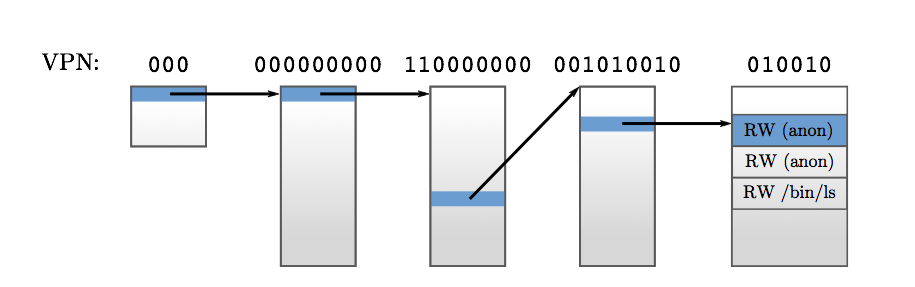
\includegraphics[width=0.8\textwidth]{figures/appedix_radixvm.png} 
  \caption*{图:基数树包含一个匿名映射映射。蓝色表示使用36位的虚页号进行查找的路径。树的最后一级为每个页面包含单独的映射元数据。}
\end{figure}

RadixVM索引数据结构类似于一个硬件页表,映射元数据存储在一个固定的深度的基数树,树的每个级别的索引由9个(或更少)的虚页号位(如图)索引。和一维数组一样,基数树只支持点查询(非范围查询)和迭代,但不像数组,RadixVM可以压缩重复的记录,
并懒惰地分配基数树的节点。从逻辑上讲,任何具有相同值的节点,将完全折叠成一个单一的记录存储在父节点中。这变形持续到树的根节点,大片的未使用的虚拟地址空间被表示成空节点,因此大范围设置为相同的值非常迅速。这种折叠在只需要很小的代价:迫使radix
tree扩展的mmap的操作可能导致多核的竞争,即使它们设计的区域不重叠。然而,这样的冲突是罕见的。

为了记录每个映射,RadixVM为每个页面映射范围的每个页面,在radix
tree中单独存储元数据。这不同于典型的设计,它们分配一个单一的元数据对象来代表一个映射(例如,在Linux的VMA结构体)。存储元数据每一页的单独副本,使在RadixVM存储的元数据相对较小,并消除共享的对象,避免mmap或munmap调用拆分或合并元数据对象,消除共享竞争。此外,映射元数据对象的设计,使最初的每一页的初始元数据对一个映射都是相同的,这意味着大的映射可以有效地创建并折成少数的几个基数树的节点。

不像典型的虚拟内存系统设计,RadixVM存储在映射元数据中存储已分配物理内存页面的指针。这在RadixVM是容易做到的,因为除去折叠,每个物理页面有一个单独的映射元数据对象。同样重要的是有这个数据结构有利于RadixVM处理TLB
shootdown。而起渐近意义下,基数树所需的空间,并不会多于硬件页表,这意味着硬件页表本身是可以被丢弃的且操作系统可以释放其内存。

为了限制基数树的内存占用,操作系统必须能够释放不再包含任何有效的映射元数据节点。为了完成这项任务,在不产生竞争的情况下,我们利用Refcache来跟踪在每个节点的引用数目。当这个计数下降到零,基数树可以从树中删除节点。

坍塌radix
tree需要引入额外的竞争,但是与饥渴的垃圾回收方案相比,快速修改映射不能造成树节点的快速删除和重建。因为一个节点必须在两个epoch以后才被真正释放,因此节点删除和重建的成本被分摊。

对比传统的平衡树,用基数树管理VM元数据允许RadixVM在非重叠地址空间范围上的并行操作,以达到完美的可扩展性。这可能造成一个潜在的更大的内存开销的成本,然而,地址空间布局往往表现出良好的局部性,并有效地压缩大的地址范围,使基数树非常适合使用在VM子系统上。

%%%%%%%%%%%%%%%%%%%%%%%%%%%%%%%%%

\subsection{TLB shootdown}

实现多核可扩展mmap或munmap操作的难点之一是每个CPU核的硬件页转换高速缓存(TLB),页面映射更改需要显式的通知(“TLB
shootdowns”)其他CPU核。因为TLB
shootdowns必须通知每个可能缓存一个被修改的页面映射的CPU,由于硬件并没有提供关于它的CPU可能有缓存一个特定的映射信息,一个保守的设计必须发送TLB
shootdown中断到所有使用相同的地址空间的CPU,这限制了VM系统的可扩展性。

通过跟踪更准确的CPU可能已经访问给定的映射的信息,RadixVM实现mmap和munmap映射元数据的更好的可扩展性。对于由软件填充TLB的体系结构,内核可以使用TLB缺失故障,准确地跟踪哪些CPU拥有一个给定的映射缓存。当以后发生mmap或munmap调用改变这种映射时,RadixVM只需要shootdown访问过这个映射的CPU核。在硬件填充TLB的(如X86)的架构上,通过使用每个核心的使用各自的页表,我们的设计可以达到同样的效果。如果应用程序中的一个线程在一个CPU核上分配,访问,和释放内存,而没有其他线程访问相同的内存区域,RadixVM不好进行TLB shootdown。


这种方法最明显的缺点是需要额外的内存维护每个CPU核的页表。但这个开销是在实际应用程序的总内存占用小。但内存不足时,内核也可以通过共享共享页表或扔掉页表来可以减少开销。


\section{讨论}

\begin{figure}[ht]
  \centering
  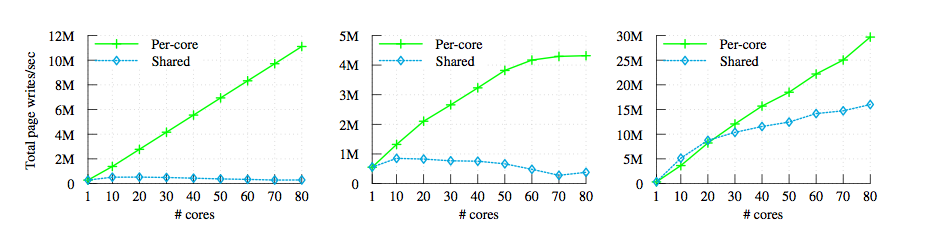
\includegraphics[width=0.8\textwidth]{figures/appedix_pagetable.png} 
  \caption*{图:使用每核单独页表和共享页表的性能对比}
\end{figure}


测试结果显示,RadixVM达到了对非重叠区域上VM操作随着CPU核数增加,完美可扩展的目标。RadixVM使用三种手段优化VM操作。有测试结果可以看出,在单核串行情况下RadixVM和Linux的性能差距在5\%以内,尽管RadixVM没有对单核情况做特殊优化。与预期一样,在多核情况下,RadixVM存储VMA元数据需要Linux两倍左右的内存。存储多核页表需要更多的内存(Metis测例下需要16倍的内存),但两种情况下,操作系统都只占内存总消耗的很小一部分。

\section{结论}
本文提出RadixVM,一个新的虚拟内存的设计,让VM密集型的多线程应用程序的性能可以达到良好的可扩展性。为了实现可扩展性,RadixVM采用三种技术:Radix
tree数据结构,Refcache,有针对性的TLB
shootdown。
使用Metis的MapReduce库和微基准测试例程,获取了一系列常见的虚拟内存使用模式。测试显示,RadixVM实现了其目标。我们希望
RadixVM的设计会激发其他的OS开发者向用户提供可扩展的虚拟内存操作原语,省却应用程序级别的解决方法。

\begin{center}
参考文献
\end{center}
[1]\hspace{15pt}Clements A T, Kaashoek M F, Zeldovich N. RadixVM: Scalable address spaces for multithreaded applications. Proceedings of Proceedings of the ACM EuroSys Conference (EuroSys 2013), Prague, Czech Republic, 2013


\

\end{appendix}

% 个人简历
% \begin{resume}

  \resumeitem{个人简历}

  xxxx 年 xx 月 xx 日出生于 xx 省 xx 县。
  
  xxxx 年 9 月考入 xx 大学 xx 系 xx 专业,xxxx 年 7 月本科毕业并获得 xx 学士学位。
  
  xxxx 年 9 月免试进入 xx 大学 xx 系攻读 xx 学位至今。

  \resumeitem{发表的学术论文} % 发表的和录用的合在一起

  \begin{enumerate}[{[}1{]}]
  \item Yang Y, Ren T L, Zhang L T, et al. Miniature microphone with silicon-
    based ferroelectric thin films. Integrated Ferroelectrics, 2003,
    52:229-235. (SCI 收录, 检索号:758FZ.)
  \item 杨轶, 张宁欣, 任天令, 等. 硅基铁电微声学器件中薄膜残余应力的研究. 中国机
    械工程, 2005, 16(14):1289-1291. (EI 收录, 检索号:0534931 2907.)
  \item 杨轶, 张宁欣, 任天令, 等. 集成铁电器件中的关键工艺研究. 仪器仪表学报,
    2003, 24(S4):192-193. (EI 源刊.)
  \item Yang Y, Ren T L, Zhu Y P, et al. PMUTs for handwriting recognition. In
    press. (已被 Integrated Ferroelectrics 录用. SCI 源刊.)
  \item Wu X M, Yang Y, Cai J, et al. Measurements of ferroelectric MEMS
    microphones. Integrated Ferroelectrics, 2005, 69:417-429. (SCI 收录, 检索号
    :896KM.)
  \item 贾泽, 杨轶, 陈兢, 等. 用于压电和电容微麦克风的体硅腐蚀相关研究. 压电与声
    光, 2006, 28(1):117-119. (EI 收录, 检索号:06129773469.)
  \item 伍晓明, 杨轶, 张宁欣, 等. 基于MEMS技术的集成铁电硅微麦克风. 中国集成电路, 
    2003, 53:59-61.
  \end{enumerate}

  \resumeitem{研究成果} % 有就写,没有就删除
  \begin{enumerate}[{[}1{]}]
  \item 任天令, 杨轶, 朱一平, 等. 硅基铁电微声学传感器畴极化区域控制和电极连接的
    方法: 中国, CN1602118A. (中国专利公开号.)
  \item Ren T L, Yang Y, Zhu Y P, et al. Piezoelectric micro acoustic sensor
    based on ferroelectric materials: USA, No.11/215, 102. (美国发明专利申请号.)
  \end{enumerate}
\end{resume}

\end{document}
